\documentclass[review,12pt,authoryear]{elsarticle}

\usepackage[T1]{fontenc}
\usepackage[utf8]{inputenc}
\usepackage{lmodern}
\usepackage{microtype}
\usepackage{amsmath,amssymb}
\usepackage{booktabs}
\usepackage{tabularx}
\usepackage{array}
\usepackage{adjustbox}
\usepackage{graphicx}
\usepackage{subcaption}
\usepackage{float}
\usepackage{xcolor}
\usepackage{enumitem}
\usepackage{siunitx}
\usepackage{url}
\usepackage{hyperref}

\definecolor{navy}{HTML}{17365D}
\definecolor{blue}{HTML}{3B6EA8}
\definecolor{green}{HTML}{2A7F86}
\hypersetup{
  colorlinks=true,
  linkcolor=navy,
  citecolor=green,
  urlcolor=blue,
  pdftitle={A Leakage-Aware Software Framework for Background-Conditioned PM2.5 Prediction under Grouped Temporal and Spatial Shifts},
  pdfauthor={Aryan Satyendra Kumar},
  pdfsubject={Temporal leakage diagnosis and leakage-aware multimodal PM2.5 estimation on TRAQID and a Taiwan fixed-camera network},
  pdfkeywords={PM2.5, multimodal estimation, temporal-context leakage, complete-date validation, leave-one-site-out, background conditioning, TRAQID, Taiwan}
}
\graphicspath{{figures_submission_final/}}
\setlist{nosep,leftmargin=*}
\setlength{\emergencystretch}{3em}
\renewcommand{\arraystretch}{1.12}
\newcolumntype{P}[1]{>{\raggedright\arraybackslash}p{#1}}
\widowpenalty=10000
\clubpenalty=10000
\displaywidowpenalty=10000
\sisetup{detect-all,group-separator={,},group-minimum-digits=4}

\newcommand{\PM}[1]{\ensuremath{\mathrm{PM}_{#1}}}
\newcommand{\pmfine}{\PM{2.5}}
\newcommand{\ugm}{\ensuremath{\mu\mathrm{g}\,\mathrm{m}^{-3}}}
\newcommand{\Rtwo}{\ensuremath{R^2}}

\journal{Environmental Modelling \& Software}

\begin{document}

\begin{frontmatter}

\title{A Leakage-Aware Software Framework for Background-Conditioned
\pmfine{} Prediction under Grouped Temporal and Spatial Shifts}

\author[nitgoa]{Aryan Satyendra Kumar\corref{cor1}}
\cortext[cor1]{Corresponding author}
\ead{kumararyan66472@gmail.com}
\address[nitgoa]{National Institute of Technology Goa, Kottamoll Plateau,
Cuncolim Municipal Area, Salcete Taluka, South Goa District, Goa 403703, India}

\begin{abstract}
Random partitioning of overlapping image sequences can overstate generalisation
in environmental machine learning. We present reusable software for raw-context
auditing, leakage-safe grouped sequences, inference-time background contracts,
grouped cross-fitting and cluster-aware uncertainty. On TRAQID, performance fell
from \Rtwo=0.950 under random windows, with 99.90\% target/context overlap, to
pooled \Rtwo=0.188 under zero-overlap complete-date evaluation; mean and median
date-wise \Rtwo{} were -5.625 and -1.042. First-10\% calibration obtained pooled
future-period \Rtwo=0.490, while mean and median date-wise \Rtwo{} remained
-1.861 and -0.583, with 3 of 16 dates positive. On Taiwan, contemporaneous
other-site background obtained \Rtwo=0.690 and the complete estimator obtained
\Rtwo=0.706 across 54 retrospectively defined later dates. Nested
leave-one-site-out evaluation retained pooled \Rtwo=0.702, mean and median
site-wise \Rtwo{} of 0.692 and 0.709, and positive skill at all six sites. The
framework therefore connects leakage diagnosis to operationally explicit,
grouped environmental prediction without claiming camera-only monitoring.
\end{abstract}

\begin{keyword}
\pmfine{} \sep temporal-context leakage \sep
grouped validation \sep background conditioning \sep multimodal estimation
\end{keyword}

\end{frontmatter}

\section{Introduction}

Roadside \pmfine{} varies across regional pollution regimes, neighbourhood
conditions and short-lived local sources. Fixed regulatory stations measure
ambient concentration accurately but provide limited spatial coverage, while
mobile sensing resolves route-level variation at the cost of substantial
temporal dependence and changing scenes. Cameras potentially encode visibility,
traffic mix and road state; atmospheric products encode broader aerosol and
meteorological conditions. Learning from these sources is therefore attractive,
but the evaluation unit must match the intended deployment question.

Temporal image studies often construct a sliding window around every target and
then randomly split the resulting windows. Two adjacent seven-frame sequences
share six frames. A model can consequently be tested on a target frame already
seen as training context, even when target rows themselves are nominally
disjoint. We use \emph{temporal-context leakage} to denote train--test sharing
of raw frames or overlapping sequence context; it is distinct from direct
target leakage. Random cross-validation is known to underestimate error
when dependence crosses partitions \citep{roberts2017cv}, and leakage remains a
major reproducibility issue in scientific machine learning
\citep{kapoor2023leakage}.

This evaluation problem motivates the modelling reformulation in this paper.
If a shuffled split allows a visual sequence model to reuse the regional
pollution regime, route and adjacent frames, a high score does not show that the
same feature system can identify local \pmfine{} conditions on a genuinely
unseen date. We therefore separate the broad pollution state from the local
departure and evaluate both only after complete dates or sites have been
isolated. The paper is consequently both diagnostic and constructive: it first
quantifies the contamination mechanism and then proposes a deployment-oriented
multimodal framework for the harder grouped-prediction problem.

This paper uses two public image--pollution datasets with complementary group
structure. TRAQID \citep{kathalkar2024traqid} is a mobile roadside campaign
spanning 20 dates and three seasons. The Taiwan subset released with the
sequential-surveillance study of Wang et al.~\citep{wang2026unified} contains
six fixed-camera monitoring sites across 276 dates. Together they support four
stages of investigation:
\begin{enumerate}
  \item diagnose raw-frame contamination produced by randomly shuffled,
        overlapping driving sequences;
  \item measure how the apparent result changes when complete collection dates
        are held out;
  \item introduce background-conditioned multimodal local refinement as a
        response to the observed date shift; and
  \item evaluate the framework under chronological future-period,
        leave-one-site-out and explicitly declared calibration-assisted tasks.
\end{enumerate}

The model is formulated as
\begin{equation}
 y_t = B_t + \Delta_t + \epsilon_t,
 \label{eq:decomposition}
\end{equation}
where $y_t$ is roadside \pmfine, $B_t$ is an external atmospheric or local
reference background, $\Delta_t$ is a learned local departure and $\epsilon_t$
contains measurement, alignment and unmodelled error. Traffic and road
variables are predictors of conditions associated with $\Delta_t$; they are
not interpreted as chemically apportioned masses.

Equation~\ref{eq:decomposition} is a governing formulation rather than a claim
that one fitted model transfers unchanged between datasets. TRAQID and Taiwan
use separate estimators, feature sets and background sources because their
sensing geometries and inference-time information differ. The shared question
is whether an inference-time background, temporal imagery and structured
context can be integrated into a useful complete system under grouped temporal
or spatial evaluation.

The novelty is not the algebraic decomposition alone, which is related to
statistical downscaling and residual correction. It is the executable contract
that connects sequence construction, background availability, grouped fitting,
overlap auditing and group-aware reporting. Separate dataset-specific estimators
implement that contract without claiming that one trained model transfers
unchanged between campaigns. The five contributions are:
\begin{enumerate}
  \item a raw-frame audit of temporal-context leakage in random T=7 evaluation;
  \item a reusable leakage-safe sequence and grouped-evaluation software workflow;
  \item an inference-time background interface for local concentration refinement;
  \item grouped temporal and spatial validation on two public datasets; and
  \item robustness and calibration-assisted analyses that define the framework's
        operating limits.
\end{enumerate}

The objective is a practical multimodal estimator rather than a camera-only
monitor: broad pollution state is supplied by the atmospheric or monitoring
background, while images and contextual variables encode local scene
conditions. The same governing design is tested across mobile and fixed-camera
settings, with zero-shot, network-assisted and calibration-assisted prediction
reported separately.

\section{Related Work}

Image-based air-quality estimation uses atmospheric attenuation, colour and
scene context as indirect aerosol cues. Luo et al. combined convolutional image
features with gradient boosting and weather/time variables
\citep{luo2020cnn}. Wang et al. used surveillance imagery with a CNN--LSTM and
reported \Rtwo=0.94 for \pmfine{} under random two-fold sequence
cross-validation \citep{wang2024surveillance}. Liu et al. reported strong
performance from a repeated fixed traffic-camera scene paired with a reference
monitor \citep{liu2024trafficcamera}. PM25Vision broadened visual benchmarking
to geographically distributed street imagery, but uses date-level AQI labels
rather than instantaneous roadside concentration \citep{han2026pm25vision}.

These results are not directly rankable: scene stability, label construction,
concentration range, aggregation interval and split unit differ. The present
study therefore compares protocols within TRAQID rather than treating published
\Rtwo{} values as a leaderboard. The central distinction is whether evaluation
measures interpolation among related sequences or prediction on a complete
unseen date.

Regional products provide a second source of information. MERRA-2 assimilates
observations into a global meteorological and aerosol reanalysis
\citep{gelaro2017merra2}; CAMS provides global atmospheric-composition analyses
and forecasts \citep{inness2019cams}. Their pixels are too coarse to replace a
roadside measurement directly, but they can anchor the broad background in
Eq.~\ref{eq:decomposition}. A nearby station can provide a more local anchor,
at the cost of changing the task to reference-assisted estimation.

This formulation sits within a longer exposure-modelling literature rather
than replacing it. Land-use regression uses traffic, land use and geographic
covariates to resolve intra-urban contrasts \citep{hoek2008lur}; statistical
downscalers calibrate coarse numerical-model output against observations
\citep{berrocal2010downscaler}; and modern exposure models combine monitors,
satellite retrievals, chemical-transport output, meteorology and land use
\citep{di2019ensemble,wei2020stet}. Those studies also show why random
sample-level validation is not equivalent to spatial or temporal transfer.
Here, imagery is tested as an incremental local predictor against explicit
atmospheric and monitoring-network baselines, not as a substitute for those
established sources.

The remaining gap is partly a software-design problem. A reported model score
does not by itself reveal whether windows were grouped before construction,
whether raw context crossed partitions, whether a background would exist at
inference, or whether preprocessing and fusion were selected outside the test
group. Existing guidance on dependence-aware validation and scientific leakage
identifies these risks \citep{roberts2017cv,kapoor2023leakage}, but they are
rarely represented as executable environmental-model contracts. The present
software makes group membership, raw-row lineage, background provenance,
selection status and group-level uncertainty first-class artifacts. This is the
specific methodological layer contributed beyond the familiar background-plus-
residual equation.

\section{Data}

\subsection{TRAQID campaign}

TRAQID is a public mobile traffic-related air-quality image dataset collected
across Hyderabad and Secunderabad, India, from October 2022 to July 2024
\citep{kathalkar2024traqid}. The platform recorded paired front and rear images
and a custom AQ Node approximately every five seconds during more than 70 hours
of driving. A Nova SDS011 measured \PM{2.5} and \PM{10}; a BME280 measured
temperature and relative humidity. The low-cost particle measurements were
calibrated against an Aeroqual S500 reference instrument in the source study.

After alignment and T=7 construction, 26,558 sequences remained across 20
dates: six monsoon dates, ten winter dates and four summer dates. Roadside
\pmfine{} ranged from 12.92 to 400.86 \ugm, with mean 66.58 and median 52.43
\ugm. Figure~\ref{fig:dataset} shows that both sequence count and target
distribution changed markedly by date. Rows are therefore numerous but are not
independent temporal replicates; the effective diversity is closer to 20 date
clusters than 26,558 independent samples.

\begin{figure}[H]
  \centering
  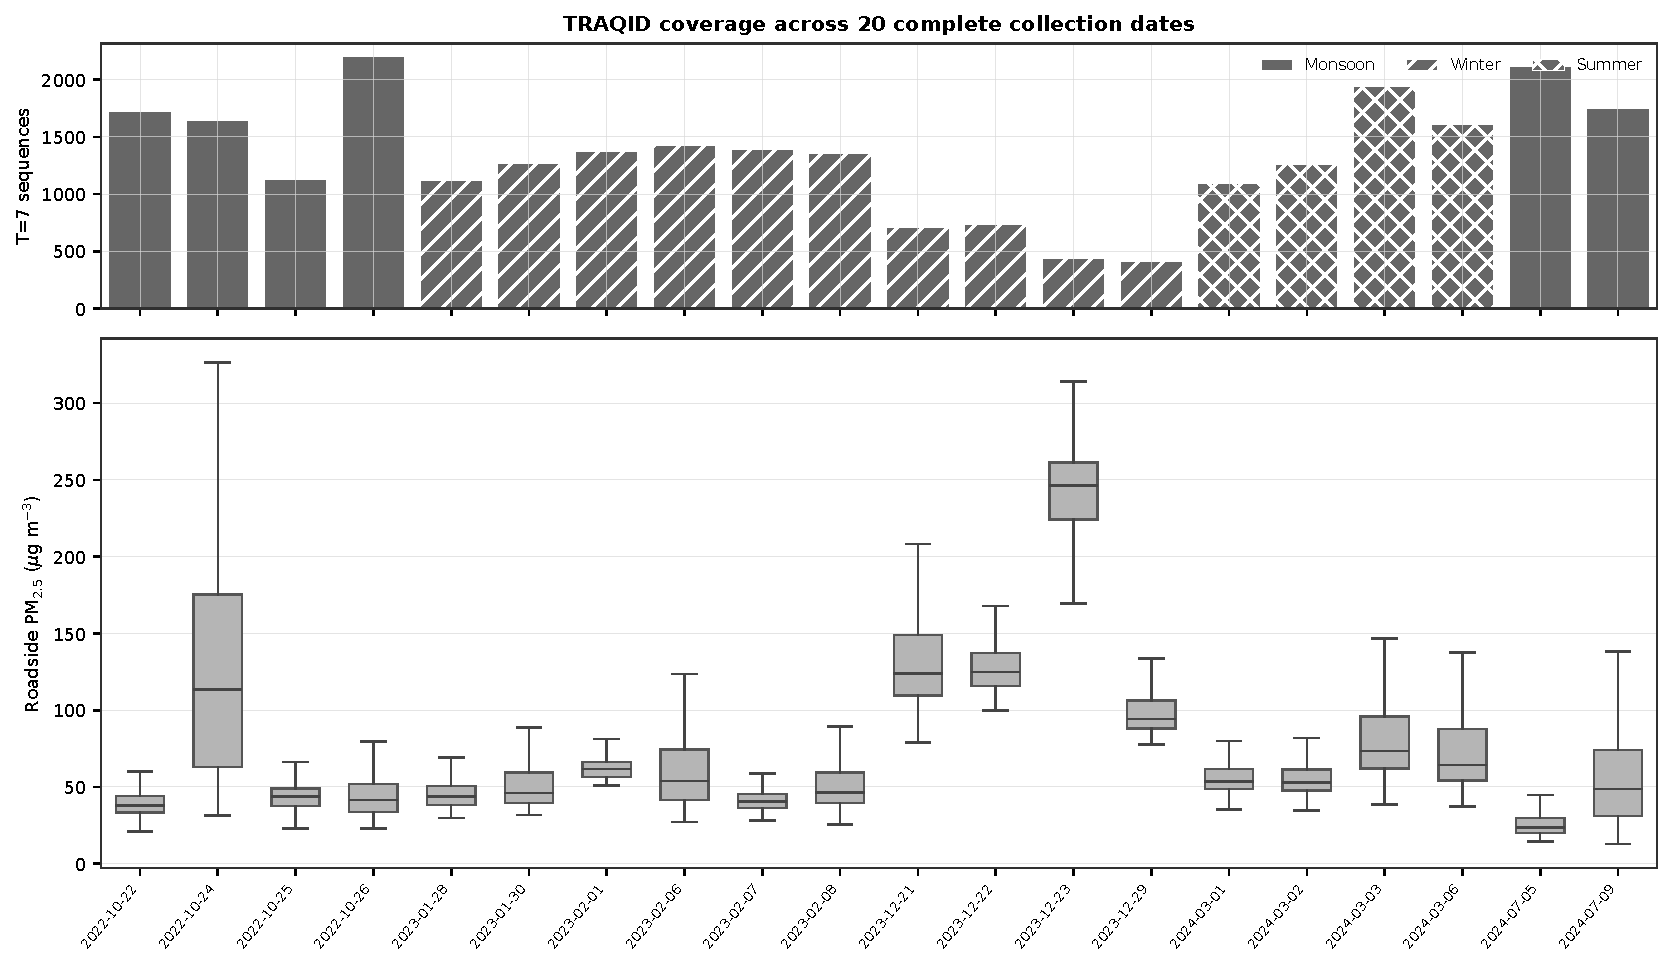
\includegraphics[width=0.98\textwidth]{Figure_01_TRAQID_coverage_and_target_distribution.pdf}
  \caption{TRAQID date coverage and roadside \pmfine{} distributions. Shading
  denotes the season labels used in the campaign-level analysis. Box plots omit
  fliers for legibility but all values are retained in modelling.}
  \label{fig:dataset}
\end{figure}

\subsection{Image, traffic and road variables}

Front and rear frames were represented with ImageNet ResNet50 global-average
pooling features \citep{he2016resnet}. Seven-frame sequences were aggregated or
encoded temporally. Structured visual features covered traffic counts, class
mix, confidence, bounding-box occupancy, near-field traffic and spatial
subregions for cars, motorcycles, auto-rickshaws, buses, trucks, bicycles and
people. Road-region variables described area, brightness, saturation,
contrast, shadow, glare, dry/brown pixels, edges, texture and a haze proxy.
The engineered T=7 table contained 102 source feature families summarized by
latest value, mean, standard deviation, minimum, maximum and change.

\subsection{Atmospheric and reference context}

Twenty-two atmospheric inputs were aligned by timestamp: MERRA-2 aerosol
components and derived \pmfine{} \citep{gelaro2017merra2,geeMerraAer}; CAMS
\PM{1}, \PM{2.5}, \PM{10} and aerosol optical-depth fields
\citep{inness2019cams,geeCamsNrt}; and ERA5-Land temperature, humidity, wind,
pressure, precipitation and solar radiation \citep{geeEra5Land}. Atmospheric
values were not fitted to the TRAQID target.

Historical OpenAQ observations were searched within 50 km of the campaign
centre \citep{openaq2026}. The retrieval artifact records 23 PM$_{2.5}$ sensors
at 13 locations. After temporal and quality filtering, usable contemporaneous
history came from OpenAQ location 8557 (``Hyderabad''), sensor 24857, supplied
by AirNow at 17.38405$^{\circ}$N, 78.45636$^{\circ}$E. OpenAQ did not expose an
instrument model for this record. The site was approximately 4.97 km from the
campaign centre. Each TRAQID timestamp was paired to the nearest hourly value
only when the absolute gap was at most 90 minutes; longer gaps were left
missing, not interpolated. Complete coverage was obtained for 16 of 20 dates
and 20,875 of 26,678 raw rows. The four uncovered dates (24 October 2022 and
6--8 February 2023) were excluded from reference-assisted comparisons. The
corresponding T=7 table contained 20,779 sequences. These results are
reference-assisted, not camera-only predictions.

\subsection{Taiwan fixed-camera monitoring network}

The second evaluation uses the Taiwan portion of the public sequential
surveillance-image air-quality dataset released by Wang et
al.~\citep{wang2026unified}. It contains hourly fixed-camera images and co-timed
\pmfine{} observations at six government monitoring locations in southern
Kaohsiung. The source publication identifies the locations as Qiaotou, Renwu,
Fengshan, Daliao, Linyuan and Xiaogang, spanning inland urban/suburban settings
and the coastal industrial belt. The redistributed folders use codes 48, 49,
50, 51, 52 and 58 in that order; these are treated as dataset codes, not assumed
to be current Ministry of Environment station identifiers. After continuity-constrained
T=7 construction, 27,084 sequences remained across 276 dates. Measured
\pmfine{} ranged from 2 to 106 \ugm{} (mean 26.28; median 26.00).

The source data cover July 2019 through April 2020 and contain
1,280$\times$720 surveillance images paired with hourly government-station
pollution records. The processed manifest retained 28,611 rows with no missing
\pmfine{} labels; availability varied from 3,743 to 5,952 rows and 169 to 273
dates per site. Table~\ref{tab:taiwan-availability} reports the site names and
retained coverage. The redistributed files do not embed latitude/longitude,
pairwise distance, station address or instrument-model fields. We therefore
report the verified district-level locations from the source publication
without reverse-engineering coordinates or monitor hardware from the numeric
folder codes.

The 276 dates were ordered chronologically before sequence construction. The
earliest 162 dates formed training, the next 52 validation and the final 54
test, producing 13,154, 6,750 and 7,180 sequences respectively. No raw image
frame occurred in more than one partition. At each target timestamp, the
monitoring-network background was the median exactly contemporaneous
(same clock-hour; zero synchronisation tolerance) \pmfine{} across
the other available sites. The target site's own measurement was excluded by
construction; consequently, the background is a network-assisted
input rather than target leakage. This task estimates one site's concentration
given images at that site and measurements elsewhere in the network. Between
one and five supporting sites were available per retained sequence (mean 4.04,
median five); on the 7,180-sequence test partition, 5,892 sequences used all
five support sites and none used fewer than two.

For a complementary spatial test, six outer folds held out one complete site
at a time. Within every outer fold, the image-correction weight was selected by
cross-validation over training sites only. All six sites were therefore scored
once as held-out spatial groups. This is network-assisted spatial transfer
within southern Kaohsiung, not sensor-free transfer to a new city.

Figure~\ref{fig:scene-examples} provides representative visual inputs from the
two evaluation domains. The mobile TRAQID views contain rapidly changing road,
traffic and illumination conditions, whereas each Taiwan camera observes a
largely fixed urban or industrial scene. These frames are shown to document the
visual domains supplied to the models; scene appearance alone is not treated as
a direct measurement of particle concentration.

\begin{figure}[H]
  \centering
  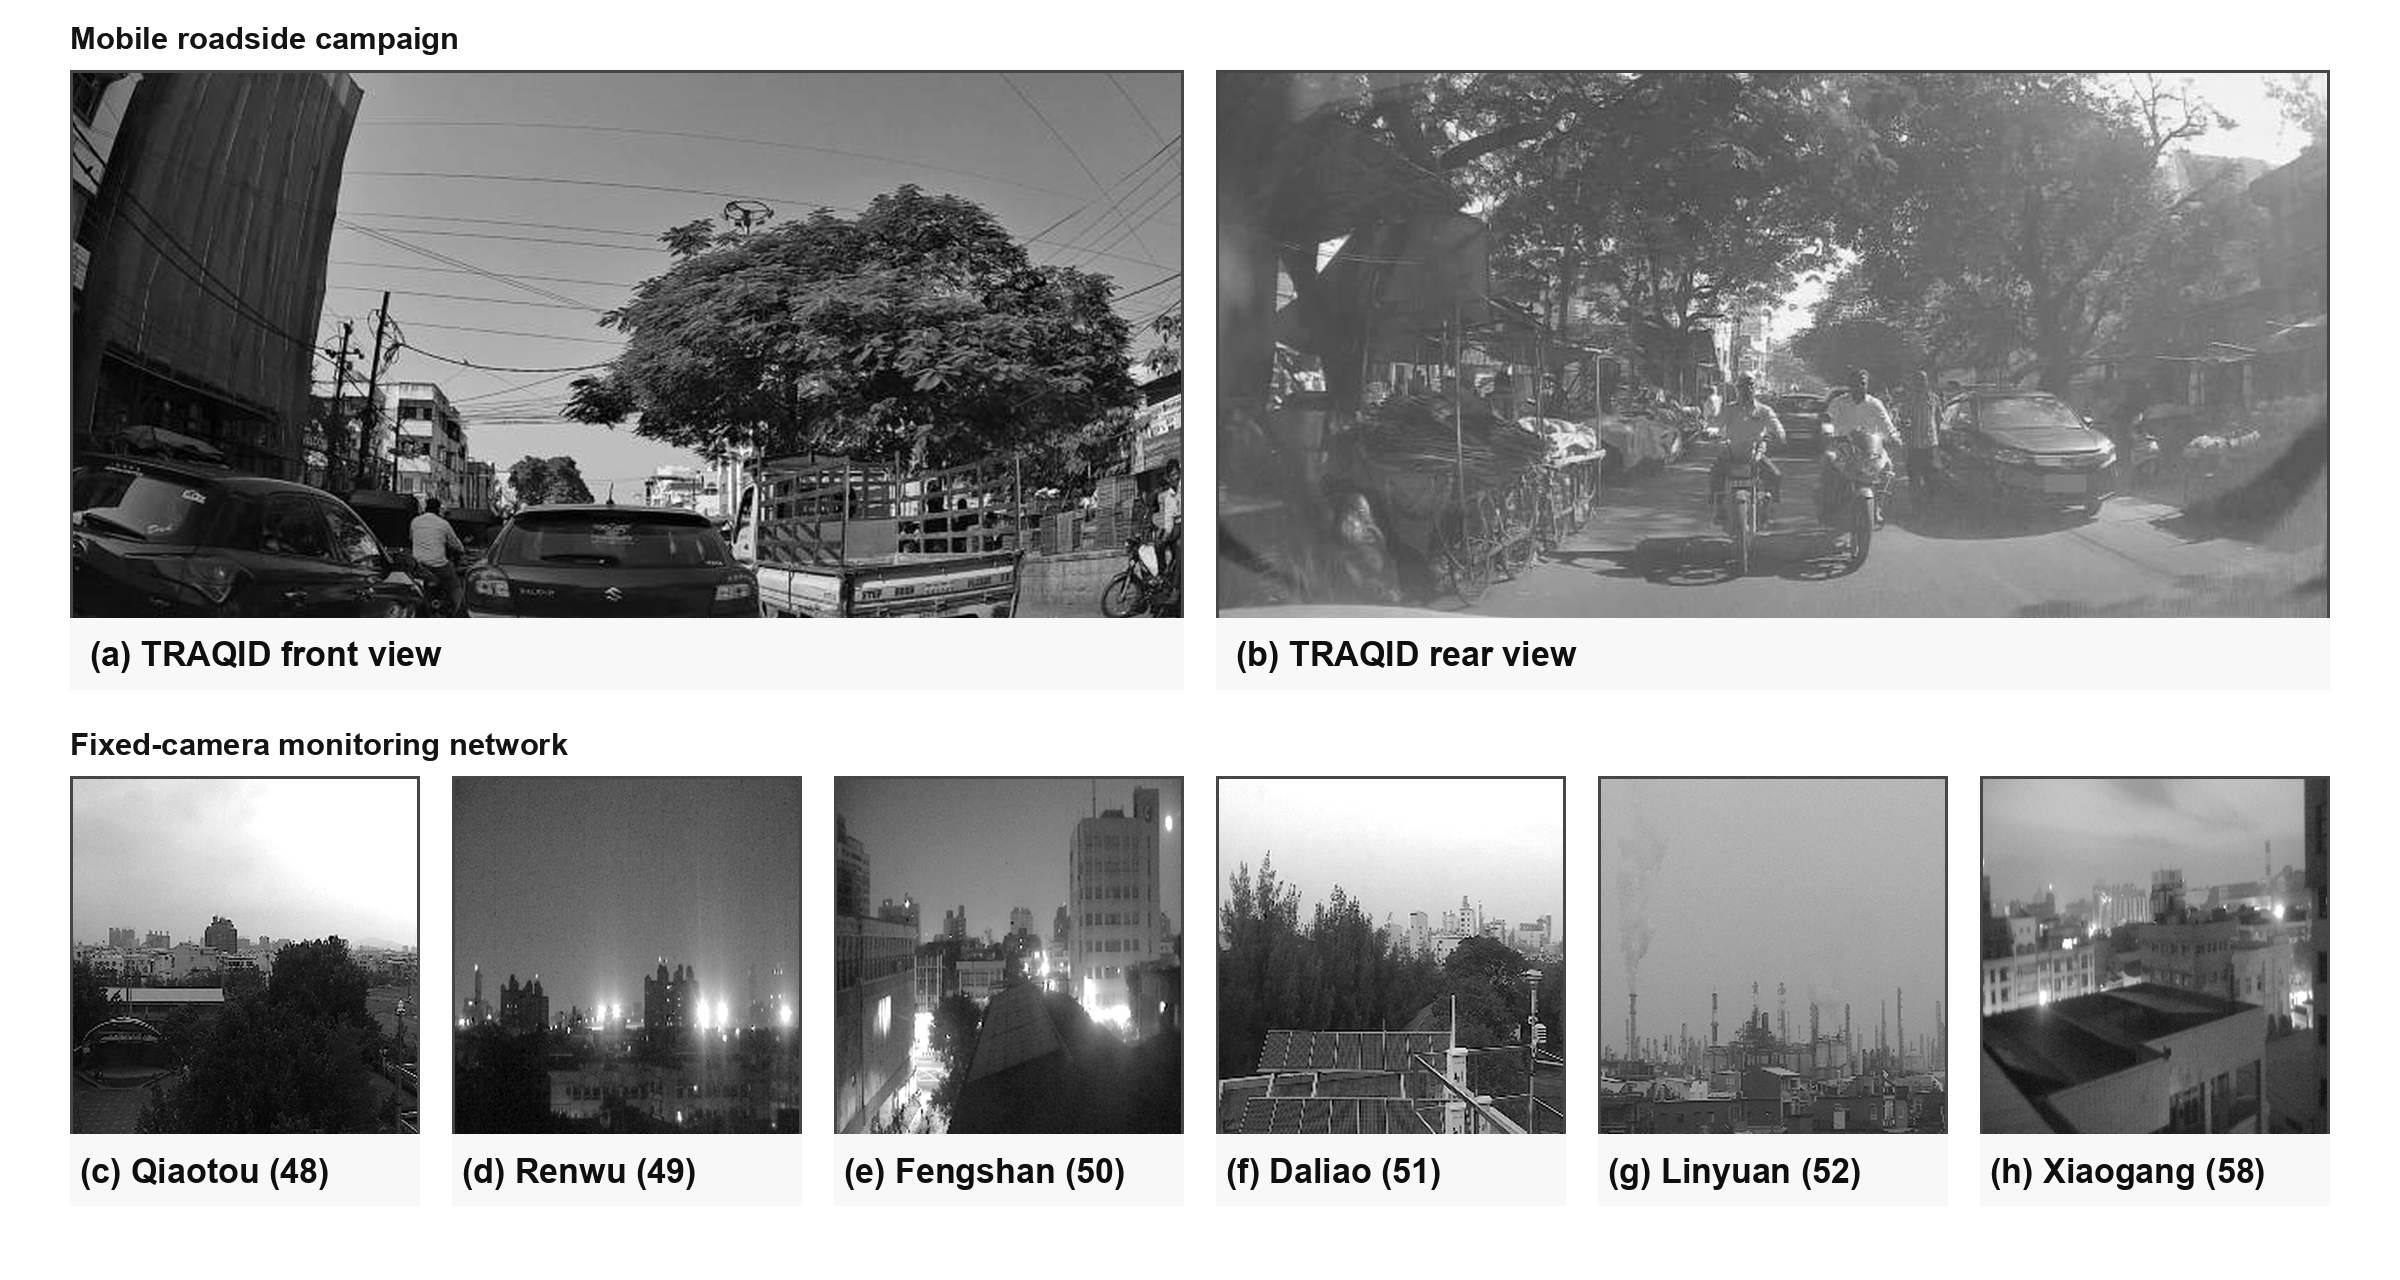
\includegraphics[width=0.99\textwidth]{Figure_02_dataset_scene_examples.png}
  \caption{Representative grayscale input frames from the public datasets.
  (a--b) Simultaneous front and rear views from the mobile TRAQID campaign
  \citep{kathalkar2024traqid}. (c--h) One fixed-camera example from each Taiwan
  monitoring location in the order Qiaotou, Renwu, Fengshan, Daliao, Linyuan
  and Xiaogang \citep{wang2026unified}. The panels illustrate the strong domain
  difference between moving roadside imagery and stationary monitoring scenes;
  they are contextual examples, not visual proxies for the associated
  \pmfine{} label. Frames were uniformly converted to grayscale and cropped
  for layout. A uniform contrast adjustment was applied; no objects or semantic
  content were added or removed. TRAQID imagery is reproduced under the source
  repository's MIT licence; Taiwan imagery is adapted under CC BY 4.0.}
  \label{fig:scene-examples}
\end{figure}

\section{Methods}

\subsection{Unified background-conditioned formulation}

Figure~\ref{fig:architecture} separates regional or network-scale background
from local estimation. A timestamp and location select an inference-time
background $B(t,s)$. A T=7 visual encoder estimates a local visual departure,
while a structured branch estimates departure from atmospheric, temporal,
traffic, road or site context available in that dataset. Validation data select
the admissible fusion; the background is added once to reconstruct the final
concentration. Predictors are covariates of one concentration and are not
interpreted as separately additive source masses.

\begin{figure}[H]
  \centering
  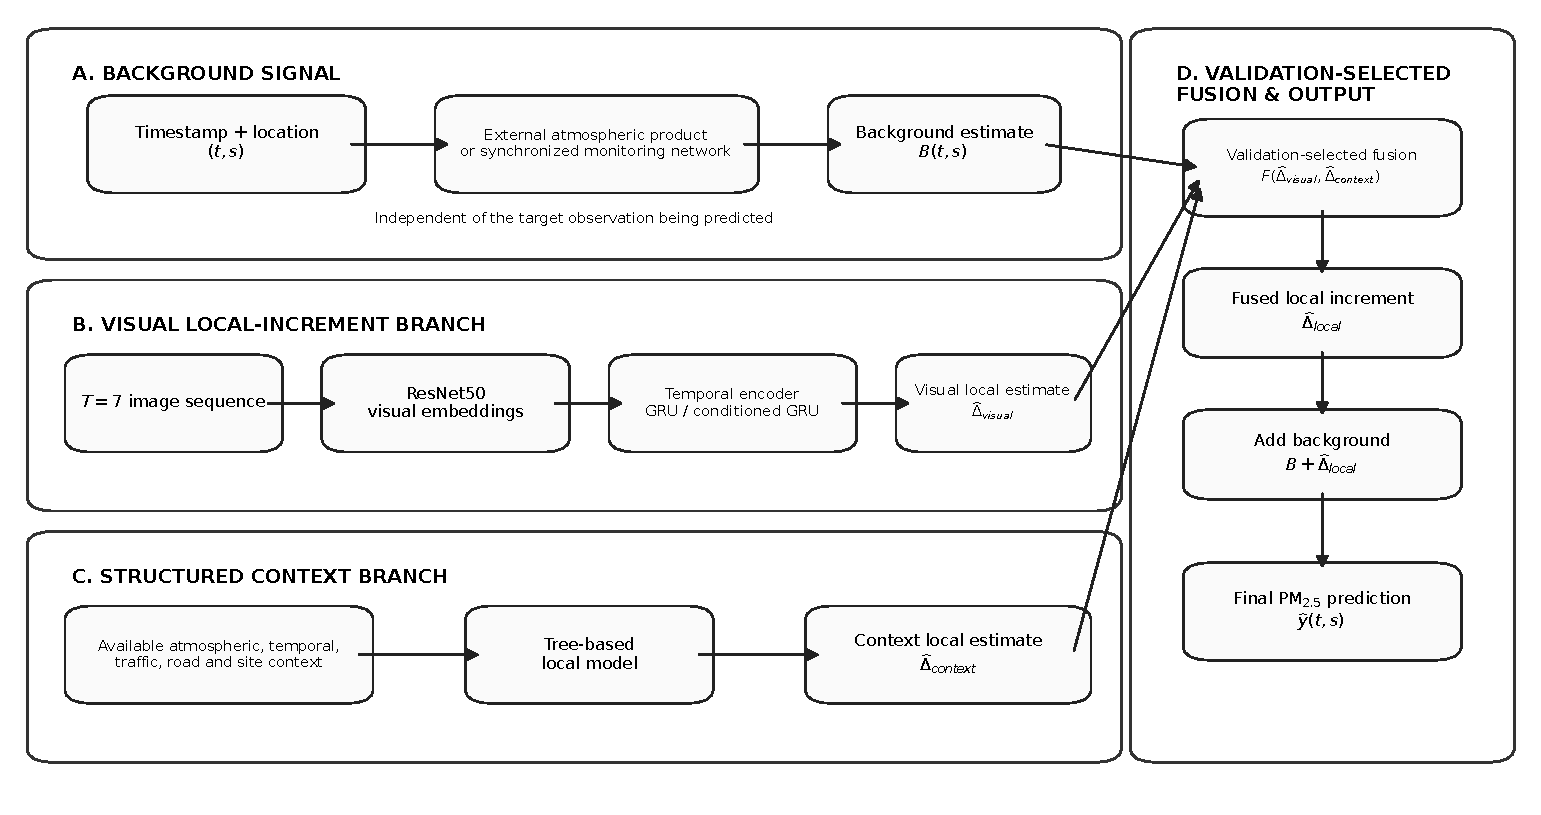
\includegraphics[width=0.99\textwidth]{Figure_03_framework_architecture.pdf}
  \caption{Shared background-conditioned architecture. TRAQID instantiates
  $B$ with MERRA-2, CAMS or a nearby monitoring station and combines temporal
  and tabular local estimates. Taiwan instantiates $B$ with the synchronized
  median of other sites, uses a cross-fitted context model and adds a bounded,
  validation-shrunk conditioned-image correction. The governing decomposition
  is shared; feature availability and the fitted fusion are dataset-specific.}
  \label{fig:architecture}
\end{figure}

The inference assumptions are deliberately explicit. In TRAQID, MERRA-2 and
CAMS are coarse atmospheric products; the OpenAQ variant additionally requires
a contemporaneous nearby monitor and is therefore reference-assisted. In
Taiwan, prediction at site $s$ requires simultaneous observations from the
other network sites, while site $s$ is excluded. These inputs are legitimate
covariates only when they would be available in the intended deployment. They
must not be compared as though they represented the same sensing burden.

\begin{table}[H]
\centering
\caption{Dataset-specific instantiations of the common decomposition. No fitted
weights are shared across datasets.}
\label{tab:instantiations}
\begin{adjustbox}{max width=\textwidth}
\begin{tabular}{P{2.0cm}P{3.1cm}P{3.4cm}P{3.2cm}P{3.6cm}}
\toprule
Dataset & Background $B$ & Learned local component & Required at inference & Excluded information \\
\midrule
TRAQID atmospheric & MERRA-2 or CAMS & Mobile image sequence + structured context & Timestamp, atmospheric products, scene covariates & Held-out-date targets \\
TRAQID assisted & Nearby OpenAQ monitor & Reference context + local covariates & Same monitor throughout the drive & Future 90\% targets \\
Taiwan network & Median of other sites & Context model + conditioned image residual & Other sites at target hour + target-site image & Target site's own observation \\
\bottomrule
\end{tabular}
\end{adjustbox}
\end{table}

\subsection{Reusable software contract and workflow}

The repository implements the framework as five composable stages rather than
as one campaign-specific training script. First, a sequence builder groups rows
before constructing windows and stores every raw-row identifier used by each
window. Second, an overlap auditor intersects those identifiers across
partitions and rejects a purported grouped evaluation when shared context is
present. Third, a background provider joins only variables declared available
at inference and records their provenance, temporal tolerance and coverage.
Fourth, local estimators are fitted inside outer groups; optional preprocessing,
residual correction and fusion are cross-fitted within the outer-training
partition. Fifth, an evaluator pools untouched outer predictions while also
reporting per-group errors, date- or site-cluster uncertainty and a machine-
readable selection-status record.

This contract makes the principal methodological safeguards testable:
\begin{equation}
 \mathcal{C}=\{G_{\mathrm{split}},I_{\mathrm{raw}},A_B,
 F_{\mathrm{inner}},E_{\mathrm{group}}\},
 \label{eq:software-contract}
\end{equation}
where $G_{\mathrm{split}}$ defines the deployment-relevant grouping,
$I_{\mathrm{raw}}$ identifies all context rows, $A_B$ declares background
availability, $F_{\mathrm{inner}}$ restricts fitting and selection to training
groups, and $E_{\mathrm{group}}$ defines pooled and grouped reporting. A new
dataset may replace the background source or local estimator while retaining
the same contract and audit outputs. The principal command-line modules and
their responsibilities are listed in Table~\ref{tab:software-workflow}; exact
commands and versioned manifests are archived with the release.

\begin{table}[H]
\centering
\caption{Reusable software stages. Paths are relative to the public repository.}
\label{tab:software-workflow}
\begin{adjustbox}{max width=\textwidth}
\begin{tabular}{P{2.5cm}P{6.0cm}P{6.6cm}}
\toprule
Stage & Representative module & Auditable output \\
\midrule
Grouped windows & \path{pipelines/image_embeddings/build_sequences.py} & Sequence manifest with groups, targets and raw-row membership \\
Background join & \path{pipelines/image_embeddings/build_traqid_reference_variants.py}; \path{pipelines/china_surveillance_aqi/build_synchronized_reference.py} & Source, matching tolerance, supporting-site count and coverage audit \\
Grouped fitting & \path{pipelines/image_embeddings/traqid_reference_innercv_lodo.py}; \path{pipelines/china_surveillance_aqi/train_conditioned_reference_gru.py} & Outer predictions, inner-selection records and fitted configuration \\
Robustness audit & \path{pipelines/image_embeddings/analyze_traqid_reviewer_metrics.py}; \path{pipelines/china_surveillance_aqi/analyze_reviewer_baselines.py} & Per-group metrics, thinning, outage and baseline sensitivity \\
Grouped inference & \path{pipelines/china_surveillance_aqi/bootstrap_conservative_visual_gain.py} & Paired date/site-cluster intervals and sufficient statistics \\
\bottomrule
\end{tabular}
\end{adjustbox}
\end{table}

\subsection{Validation protocols}

Table~\ref{tab:protocols} separates the evaluation questions. Random T=7
windows retain the published-style diagnostic but do not measure deployment.
LODO holds one complete date out, fits preprocessing and estimators on the
other dates, and concatenates each untouched outer-test prediction for pooled
metrics. The calibration protocol begins from these frozen predictions, uses
the earliest 10\% of the held-out date as adaptation data, removes every future
sequence sharing any raw row with adaptation, and evaluates the remainder.

\begin{table}[H]
\centering
\caption{Evaluation protocols and their permitted interpretation.}
\label{tab:protocols}
\begin{adjustbox}{max width=\textwidth}
\begin{tabular}{P{3.0cm}P{3.2cm}P{2.7cm}P{5.3cm}}
\toprule
Protocol & Split unit & Direct frame overlap & Interpretation \\
\midrule
Random overlapping T=7 & Sequence after window construction & Severe & Same-distribution diagnostic only \\
20-date LODO & Complete collection date & None & Zero-shot cross-date evaluation \\
16-date reference LODO & Complete reference-covered date & None & Zero-shot, reference-assisted evaluation \\
10\% adaptation / future 90\% & Chronological within held-out date, exact raw-row purge & None & Calibration-assisted future-period prediction \\
Taiwan chronological 60/20/20 & Complete dates assigned before T=7 construction & None & Retrospective future-period evaluation \\
Taiwan nested LOSO & Complete monitoring site; inner training-site CV & None & Network-assisted spatial transfer \\
Oracle corrections & Entire evaluated date & Uses all test targets & Diagnostic ceiling only \\
\bottomrule
\end{tabular}
\end{adjustbox}
\end{table}

\subsection{Random-window architecture and overlap audit}

The random benchmark used an external MERRA-2 background and two local
branches. A ResNet50--GRU T=7 temporal branch predicted the local increment and
received cross-fitted Random Forest residual correction
\citep{he2016resnet,cho2014gru,breiman2001rf}. An ExtraTrees branch used 631
multiscale atmospheric, weather, traffic and road predictors
\citep{geurts2006extratrees}. A validation-trained conditional gate combined
the branch predictions. Train, validation and test targets were disjoint, but
the raw frame identifiers composing every sequence were audited across
partitions.

\subsection{Complete-date background-decomposition models}

For full 20-date LODO, MERRA-2 supplied $B_t$. Local ExtraTrees models compared
nonvisual context, nonvisual plus images, nonvisual plus structured visual and
all modalities. Image features were reduced by train-only randomised PCA. All
imputation, scaling, PCA and model fitting were restricted to outer-training
dates.

For the 16 reference-covered dates, the OpenAQ measurement was forced as
$B_t$. Reference-context variables included the current level, T=7 mean,
standard deviation, change and slope, plus contrasts against CAMS and MERRA-2.
The strongest zero-shot branch used reference context, meteorology, time and
atmospheric variables. Images and structured visual variables were retained as
matched ablations rather than assumed to be beneficial.

Both TRAQID grouped runners used date-balanced sample weights and median
imputation with missingness indicators. Local ExtraTrees models used 300 trees,
minimum leaf size 8 and \texttt{max\_features}=0.7. ImageNet ResNet50 frame
embeddings were reduced by train-only randomised PCA to at most 48 components;
latest, mean, standard deviation and first-to-last change over T=7 were then
concatenated. The reference-assisted fusion used four inner date-grouped folds
and a simplex step of 0.05. The chronological meta-calibrator standardized its
single early-residual feature and selected ridge
$\alpha\in\{0.01,0.1,1,10,100\}$ by leave-one-date-out cross-validation among
the other 15 dates. All random seeds were 42 unless a deterministic fold offset
was recorded by the runner.

\subsection{Taiwan monitoring-network and conditioned-image model}

For target site $s$, the background $B(t,s)$ was the contemporaneous median of
the other available sites. A six-variable context vector contained $B(t,s)$,
the contributing-site count and cyclic hour and day-of-year terms. ExtraTrees
predicted the local increment $y-B$. Training predictions were cross-fitted by
site before constructing the neural correction target, preventing the image
branch from learning an in-sample residual of the context model.

Each T=7 image sequence was represented by ResNet50 embeddings. A context
encoder generated feature-wise linear modulation parameters for a one-layer GRU
with hidden width 128. The network predicted the remaining correction after the
context branch; a hyperbolic tangent bounded its magnitude at 15 \ugm. The
final estimator was
\begin{equation}
 \widehat y(t,s)=B(t,s)+\widehat\Delta_{\mathrm{ctx}}(t,s)
                 +\alpha\,\delta_{\mathrm{img}}(t,s).
 \label{eq:taiwan}
\end{equation}
For the chronological experiment, checkpoint and $\alpha=0.30$ were selected
on the 52-date validation partition and frozen before the 54-date test was
scored. For outer leave-one-site-out evaluation, $\alpha\in[0,0.30]$ in steps
of 0.02 was selected separately using cross-validation among outer-training
sites; the held-out site's targets were never used for selection.

The context ExtraTrees model used 400 trees, minimum leaf size 10 and
\texttt{max\_features}=0.8. The conditioned image network used a 256-dimensional
projection of frozen ResNet50 embeddings, a one-layer GRU with hidden width
128, dropout 0.3 and a correction bound of 15 \ugm. It was optimised with
AdamW (learning rate $10^{-4}$, weight decay $10^{-4}$), Huber loss with
$\delta=3$, correction penalty 0.005, batch size 64, at most 80 epochs and
patience 12. Checkpoint and correction weight were selected exclusively on the
declared validation groups. \ref{app:provenance} records exact
artifacts and selection status.

After the frozen chronological test had been inspected, an exploratory network
ablation compared learned spatial and lagged spatiotemporal backgrounds and a
validation-selected nonnegative ensemble. Its split controls remain valid, but
its test values are labelled exploratory and are not used as confirmatory
headline results.

\subsection{Chronological calibration-assisted model}

For the TRAQID calibration-assisted experiment, the earliest 10\% of each held-out
date was assigned to adaptation;
ties at the boundary timestamp remained together. Every later sequence whose
seven raw rows intersected adaptation was purged. This removed six boundary
sequences per date (96 total), leaving 18,554 future sequences after 2,129
adaptation sequences.

Let $e_d^{\mathrm{early}}$ be the median residual $y-\hat y$ in the adaptation
segment and $e_d^{\mathrm{future}}$ the mean residual in the later segment. For
target date $d$, a ridge mapping
\begin{equation}
 \widehat e_d^{\mathrm{future}} =
 f_{-d}\!\left(e_d^{\mathrm{early}}\right)
 \label{eq:meta}
\end{equation}
was fitted using the other 15 dates only. Ridge strength was selected by
leave-one-date-out cross-validation inside those 15 dates. The calibrated
prediction was
\begin{equation}
 \hat y_{d,t}^{\mathrm{cal}}=\hat y_{d,t}+\widehat e_d^{\mathrm{future}}.
 \label{eq:calibration}
\end{equation}
No target from the future 90\% of date $d$ entered $f_{-d}$, its
hyperparameter selection or the frozen base model. Direct mean, median and
affine corrections fitted only on the first 10\% were included as controls.

\subsection{Metrics and uncertainty}

We report MAE, RMSE, bias and pooled \Rtwo{} after concatenating outer-test
predictions. Because within-date variance differs markedly, per-date \Rtwo{}
can be unstable; rather than omit it, we report its mean, median and number of
positive dates alongside macro-averaged date MAE/RMSE. Date-centred \Rtwo{}
subtracts the observed and predicted mean within each date before pooling and
therefore measures within-date shape independently of between-date offsets.
A deterministic non-overlapping sensitivity retains every seventh target in
time order within each date, so retained T=7 windows do not share raw frames.
TRAQID date-cluster uncertainty resampled the 16 complete dates with replacement
5,000 times, retaining every row within a sampled date. Taiwan uncertainty used
5,000 paired resamples of the 54 chronological test dates and, separately,
20,000 paired resamples of the six outer test sites. Percentile intervals
therefore measure sensitivity to the relevant grouped units rather than treating
dense sequences as independent samples. All analyses used fixed seed 42 and
scikit-learn \citep{pedregosa2011sklearn}.

The primary endpoint for TRAQID was matched future-90\% RMSE after
calibration, compared with the uncalibrated prediction on exactly the same
sequences. The primary Taiwan endpoint was chronological-test RMSE relative to
the prespecified contemporaneous other-site median. Pooled \Rtwo{}, grouped
\Rtwo{} and correlation are secondary descriptors. This ordering was fixed for
the manuscript revision to avoid selecting the most favourable metric after
inspection.

The study was developed iteratively. The random-window reproduction, backbone
comparisons and several background variants were exploratory. The grouped
protocols, exclusion of target-site measurements, chronological partitions and
primary matched comparisons were then evaluated from preserved split manifests
and prediction files. \ref{app:provenance} distinguishes diagnostic,
grouped, assisted and post-hoc results. A future prospective study should freeze
the full analysis plan before acquiring target labels.

\section{Results}

The results follow the study logic. Section~5.1 diagnoses the shuffled-window
failure mode. Sections~5.2--5.4 then evaluate the proposed
background-conditioned framework under chronological, held-out-site and
complete-date shifts, and Section~5.5 tests the explicitly assisted prediction
setting. Component-level comparisons are retained in the appendix so that the
main sequence remains diagnosis, reformulation and grouped validation.

\subsection{Protocol audit separates interpolation from grouped prediction}

The exact random-window conditional architecture achieved MAE 5.36 \ugm,
RMSE 10.29 \ugm{} and pooled \Rtwo=0.950 on 3,983 test sequences. However,
24,546 of 26,678 raw rows occurred in more than one partition, 18,159 raw rows
overlapped train and test, and 3,979 of 3,983 test targets (99.90\%) had already
appeared as training context. The result demonstrates reproducible interpolation
under the shuffled-window protocol, not future-date prediction.

The same audit applied to random two-fold sequence cross-validation---the
evaluation pattern used by representative surveillance-image studies---found
that 74.81\% of test sequences shared at least six of seven raw frames with a
training sequence and only 0.01\% had zero overlap. This does not establish
that every published image-based result is contaminated; it establishes that
overlapping-window protocols are structurally vulnerable unless raw-frame
separation is verified explicitly.

\begin{table}[H]
\centering
\caption{Frame-overlap audit for representative TRAQID protocols.}
\label{tab:overlap}
\begin{adjustbox}{max width=\textwidth}
\begin{tabular}{lrrrr}
\toprule
Protocol & Eval $n$ & Mean max overlap & Share $\geq6/7$ & Share zero \\
\midrule
Random 70/15/15 & 3,983 & 5.899 & 90.91\% & 0.00\% \\
Random two-fold & 13,279 & 5.667 & 74.81\% & 0.01\% \\
Time-balanced purged & 6,691 & 0.000 & 0.00\% & 100.00\% \\
Complete-date & 5,462 & 0.000 & 0.00\% & 100.00\% \\
Chronological 10\% adaptation & 18,554 & 0.000 & 0.00\% & 100.00\% \\
\bottomrule
\end{tabular}
\end{adjustbox}
\end{table}

\subsection{Grouped multimodal estimation across dates and sites}

The Taiwan experiment supplied a stronger fair test because it contained 276
dates and six synchronized sites. Figure~\ref{fig:taiwan-protocol} documents the
partition audit. Dates were assigned before windows were constructed, raw-frame
overlap across train, validation and test was zero, and a target site's reading
never contributed to its own background. Checkpoint and image weight were fixed
on validation before the reported frozen scoring, but the dataset belonged to a
broader iterative research programme; this is therefore retrospective grouped
validation rather than prospective confirmation.

\begin{figure}[H]
  \centering
  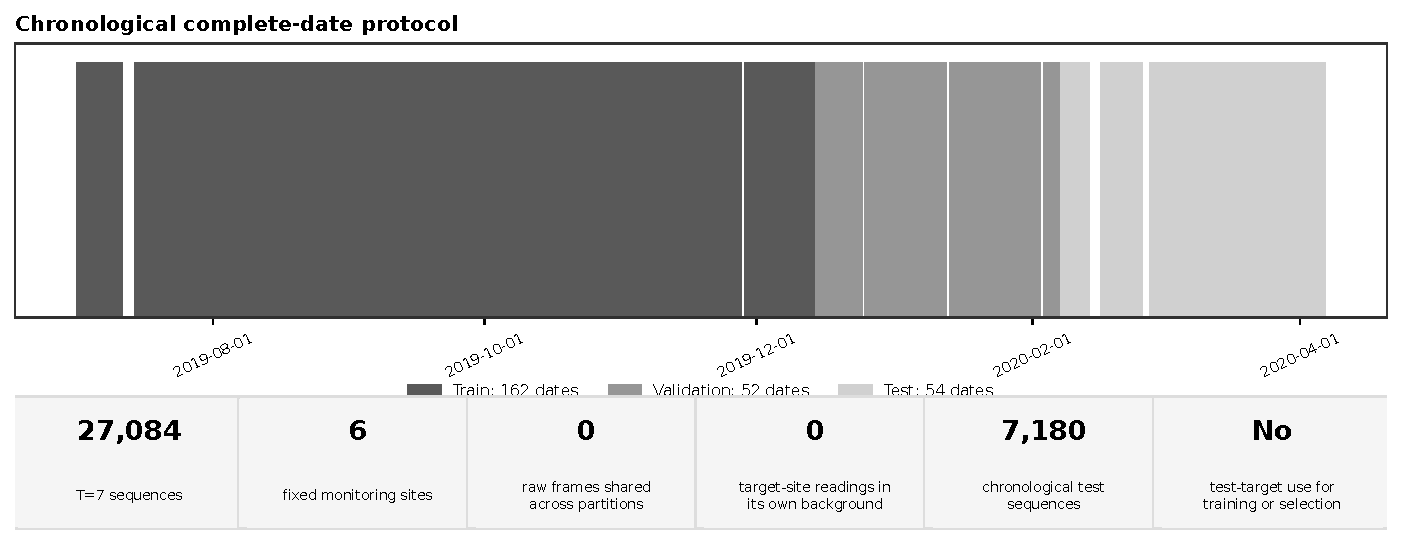
\includegraphics[width=0.98\textwidth]{Figure_04_protocol_and_leakage_audit.pdf}
  \caption{Taiwan chronological protocol and leakage audit. The earliest 162
  dates train the model, 52 subsequent dates select it and the final 54 dates
  provide 7,180 test sequences. All reported counts are generated from the
  frozen sequence manifest and split audit.}
  \label{fig:taiwan-protocol}
\end{figure}

The primary Taiwan endpoint was chronological-test RMSE relative to the
prespecified other-site median. On the future period, the synchronized network
background alone obtained MAE 4.70 \ugm, RMSE 6.61 \ugm{} and
\Rtwo=0.690. The background-plus-context-plus-conditioned-image model
improved these to 4.58, 6.44 and 0.706, respectively (Table~\ref{tab:taiwan}).
Its Pearson and Spearman correlations were 0.846 and 0.868. Date-block
resampling estimated a median RMSE reduction of 0.172 \ugm{} (95\% interval
0.082--0.251) and an \Rtwo{} gain of 0.016 (0.007--0.026); 49 of 54 dates had
positive within-date \Rtwo{} and RMSE decreased on 41 dates.

Transparent network baselines clarify where this skill originates
(Table~\ref{tab:taiwan-baselines}). A training-only target-site/hour
climatology failed on the future period (\Rtwo=-0.116), and delaying the
other-site median by one hour reduced \Rtwo{} to 0.647. Contemporaneous
other-site mean and median baselines reached 0.696 and 0.690. Relative to the
median, the conditioned-image estimator improved MAE by 0.124 \ugm,
RMSE by 0.172 \ugm{} and \Rtwo{} by 0.016 in 5,000 paired complete-date
resamples; all three 95\% intervals excluded zero. Removing any one support
station changed median-background RMSE from 6.61 to 6.68--6.81 \ugm, showing
moderate rather than catastrophic single-station sensitivity.

\begin{table}[H]
\centering
\caption{Transparent baselines on the identical frozen 54-date Taiwan test
partition. The target site's contemporaneous observation is absent from every
network predictor.}
\label{tab:taiwan-baselines}
\begin{adjustbox}{max width=\textwidth}
\begin{tabular}{lrrrr}
\toprule
Model & MAE & RMSE & Pooled \Rtwo & Coverage \\
\midrule
Training mean & 10.035 & 12.717 & -0.146 & 100.0\% \\
Target-site/hour climatology & 9.923 & 12.550 & -0.116 & 100.0\% \\
Other-site median, one-hour lag & 5.050 & 7.061 & 0.647 & 99.85\% \\
Other-site contemporaneous median & 4.704 & 6.613 & 0.690 & 100.0\% \\
Other-site contemporaneous mean & 4.718 & 6.553 & 0.696 & 100.0\% \\
Frozen conditioned-image estimator & \textbf{4.580} & \textbf{6.442} & \textbf{0.706} & 100.0\% \\
\bottomrule
\end{tabular}
\end{adjustbox}
\end{table}

The network-assisted spatial result was consistent. Nested leave-one-site-out evaluation scored
27,019 sequences and obtained pooled MAE 4.82 \ugm, RMSE 6.46 \ugm{} and
\Rtwo=0.702. Every held-out site had positive \Rtwo{} (0.534--0.778), with
mean and median site-wise \Rtwo{} of 0.692 and 0.709. Fusion weights were
selected only within the training sites, so the complete framework was tested
without using the outer site's labels. Detailed component and weight
sensitivity is reported in \ref{app:component-audit}; the principal
result is that the combined estimator retained positive skill under both
chronological and held-out-site evaluation. The other-site network already
carried most of the predictive signal; conditioned imagery provided a small,
statistically measurable refinement rather than replacing that network.
At the six-site inference level, the increment over the context-only model was
less certain: the pooled \Rtwo{} gain was 0.0038 and its paired site-cluster
95\% interval was -0.0045--0.0120. Corresponding MAE and RMSE reductions were
0.0556 \ugm{} (-0.0385--0.1577) and 0.0412 \ugm{}
(-0.0447--0.1256). These intervals use the six sites as the resampling units;
20,000 resamples improve numerical stability but do not increase the number of
independent spatial clusters.

\begin{table}[H]
\centering
\caption{Taiwan grouped framework evaluation. Chronological rows share one
frozen future-period test set. LOSO rows concatenate six outer test sites;
fusion is selected only by inner training-site cross-validation. Detailed
component rows are reported in \ref{app:component-audit}.}
\label{tab:taiwan}
\begin{adjustbox}{max width=\textwidth}
\begin{tabular}{llrrrrl}
\toprule
Protocol & Model & $n$ & MAE & RMSE & Pooled \Rtwo & Status \\
\midrule
Chronological & Other-site network background & 7,180 & 4.704 & 6.613 & 0.690 & Frozen baseline \\
Chronological & Background + context & 7,180 & 4.786 & 6.666 & 0.685 & Frozen component \\
Chronological & Background + context + conditioned image & 7,180 & \textbf{4.580} & \textbf{6.442} & \textbf{0.706} & Frozen test \\
\midrule
Nested LOSO & Other-site network background & 27,019 & 4.868 & 6.604 & 0.689 & Outer test \\
Nested LOSO & Background + context & 27,019 & 4.873 & 6.501 & 0.699 & Outer test \\
Nested LOSO & Conservative conditioned image & 27,019 & \textbf{4.818} & \textbf{6.460} & \textbf{0.702} & Inner-CV selected \\
\bottomrule
\end{tabular}
\end{adjustbox}
\end{table}

\begin{figure}[H]
  \centering
  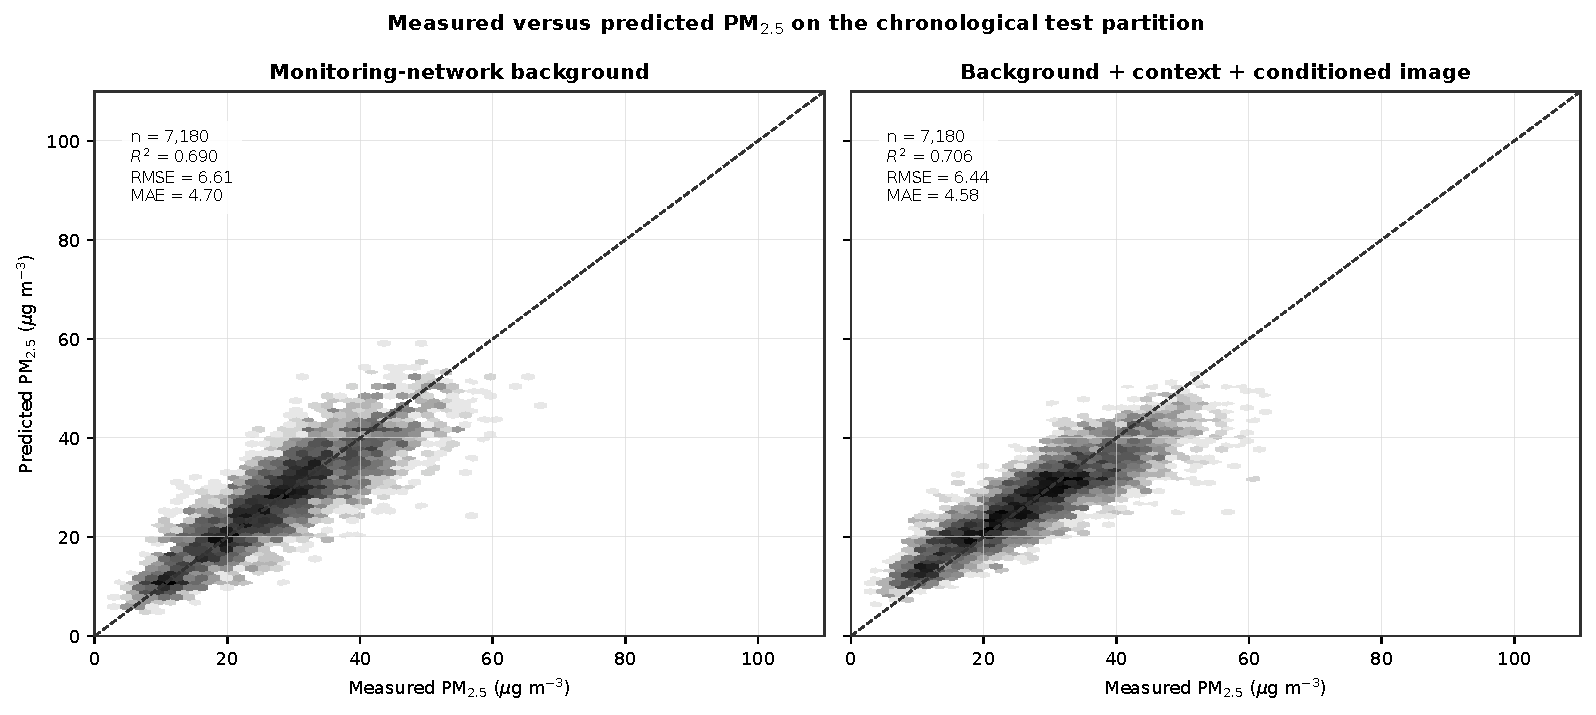
\includegraphics[width=0.98\textwidth]{Figure_05_measured_vs_predicted.pdf}
  \caption{Measured versus predicted Taiwan \pmfine{} on the chronological
  54-date test period. Both panels use identical 7,180 sequences and axes. The
  conditioned model reduces aggregate error but still underestimates sparse
  high-concentration observations.}
  \label{fig:taiwan-scatter}
\end{figure}

\begin{figure}[H]
  \centering
  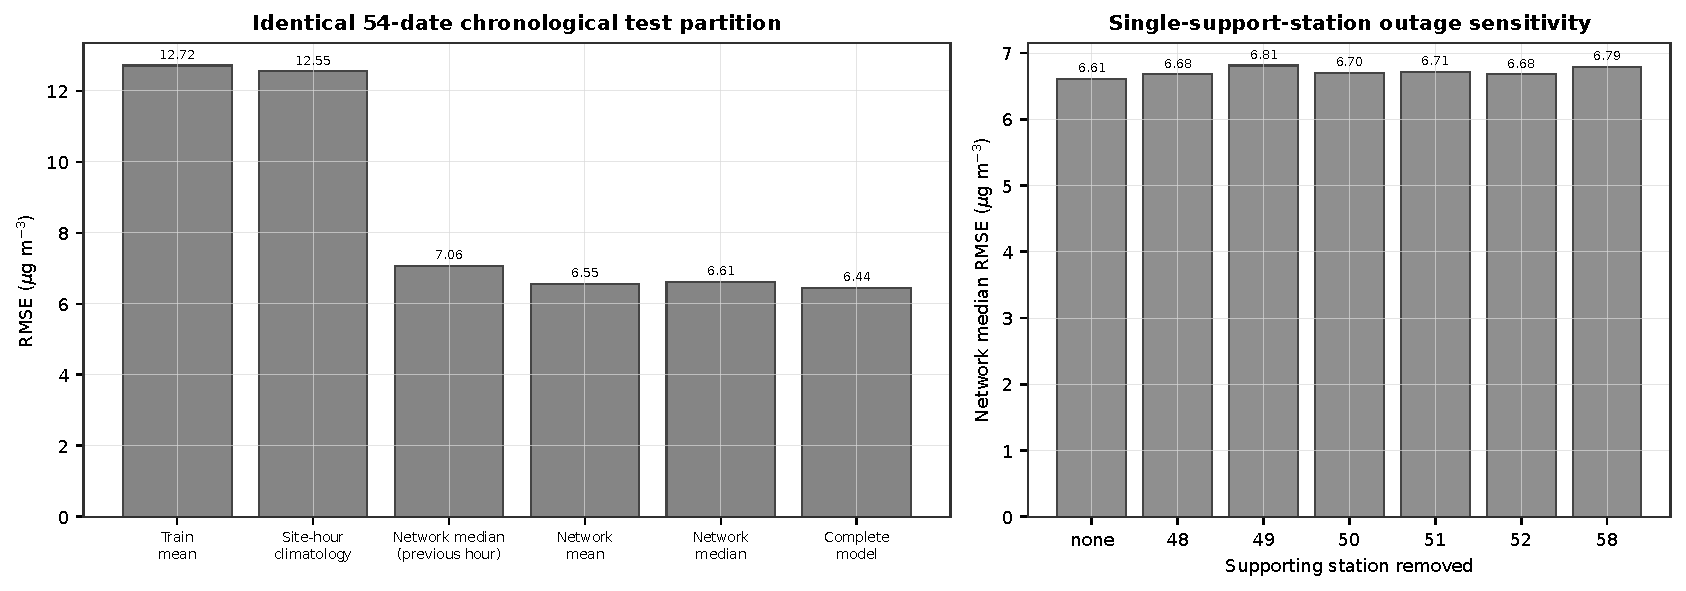
\includegraphics[width=0.98\textwidth]{Figure_06_baselines_and_outages.pdf}
  \caption{Monitoring-network baseline and reliability audit. Left: RMSE on
  the identical 54-date chronological test partition. Right: network-median
  RMSE after removing one support site at a time.}
  \label{fig:taiwan-baselines-outages}
\end{figure}

\begin{figure}[H]
  \centering
  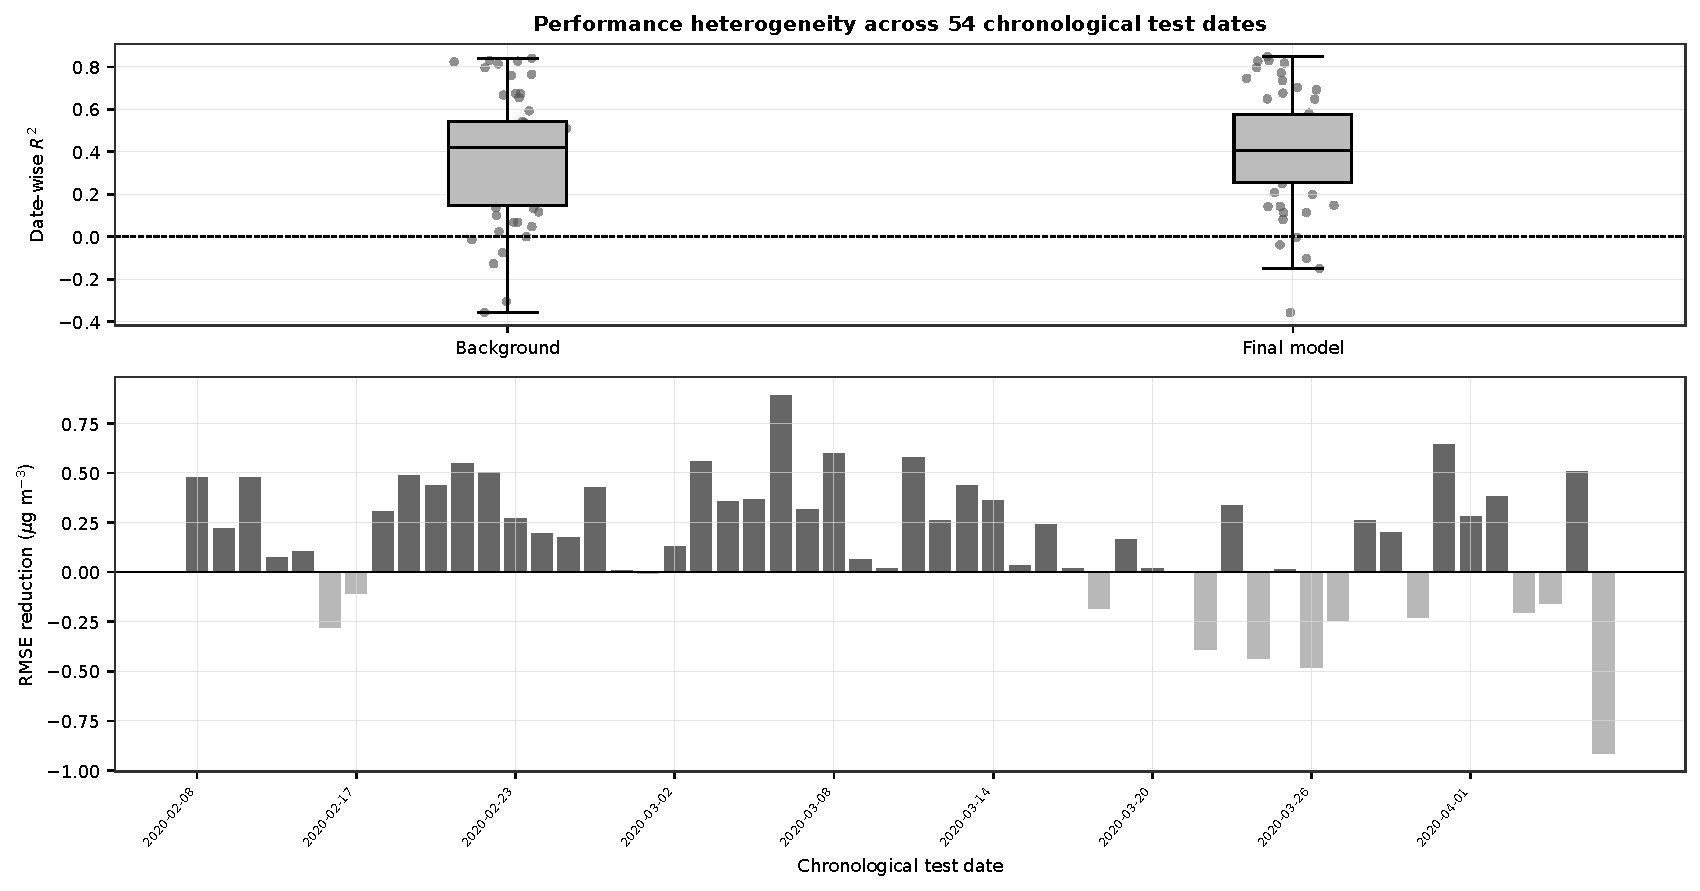
\includegraphics[width=0.92\textwidth]{Figure_07_datewise_robustness.pdf}
  \caption{Taiwan complete-date robustness on the chronological test.
  The visual correction does not improve every date.}
  \label{fig:taiwan-datewise}
\end{figure}

\begin{figure}[H]
  \centering
  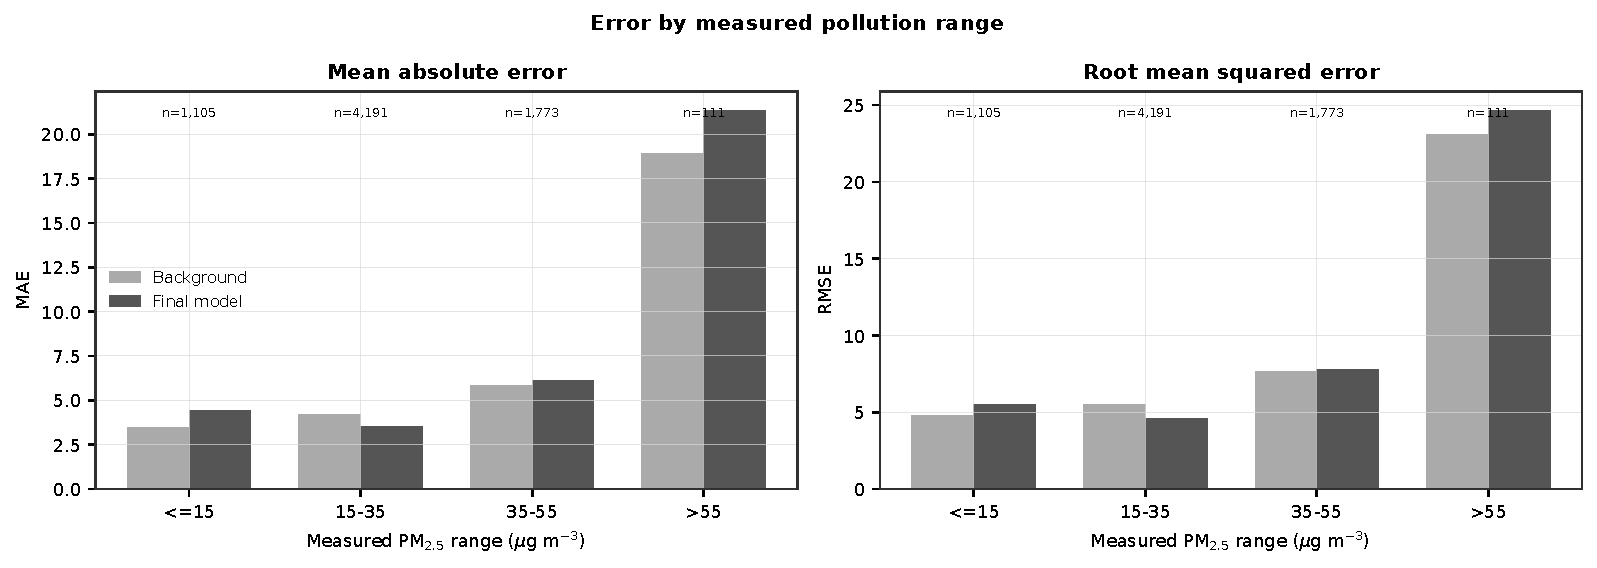
\includegraphics[width=0.92\textwidth]{Figure_08_pollution_range_performance.pdf}
  \caption{Taiwan concentration-stratified error. The conditioned image
  improves aggregate performance and the 15--35 \ugm{} stratum, but not every
  concentration range; high-concentration observations remain difficult.}
  \label{fig:taiwan-range}
\end{figure}

\begin{figure}[H]
  \centering
  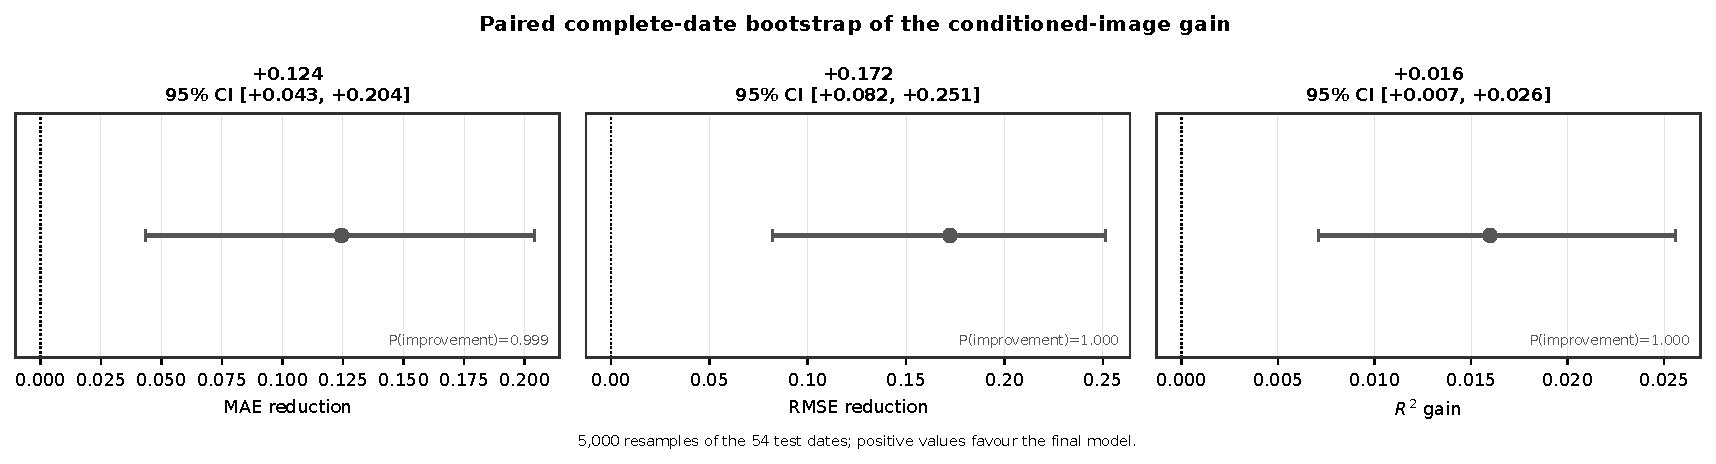
\includegraphics[width=0.98\textwidth]{Figure_09_date_block_bootstrap_gain.pdf}
  \caption{Paired complete-date bootstrap for the frozen Taiwan model relative
  to the other-site monitoring-network background. Positive reduction denotes
  lower error. Intervals are percentile 95\% intervals from 5,000 resamples
  of all 54 chronological test dates.}
  \label{fig:taiwan-bootstrap}
\end{figure}

\subsection{Complete-date TRAQID evaluation}

Table~\ref{tab:main} shows the validation ladder.
On all 20 dates, the strongest zero-shot LODO configuration combined nonvisual
and image context, obtaining MAE 28.53 \ugm, RMSE 42.14 \ugm{} and pooled
\Rtwo=0.188. This protocol transition established the need for background
conditioning under date isolation. The 16-date reference-assisted model improved
MAE to 23.94 \ugm, RMSE to 36.23 \ugm{} and pooled \Rtwo{} to 0.361. On the
matched future-90\% subset, calibration-assisted prediction further increased pooled
\Rtwo{} from 0.371 to 0.490. The oracle diagnostics reached 0.582 and 0.663,
but use the full evaluated date and therefore represent ceilings, not inference-realistic
performance. Rows with different coverage are not treated as paired tests.

Pooled skill did not imply stable within-date tracking
(Table~\ref{tab:traqid-grouped}). The 20-date model had mean and median
date-wise \Rtwo{} of -5.625 and -1.042, with three positive dates; its
date-centred \Rtwo{} was -0.071. The calibrated future-90\% model improved
macro date RMSE to 27.80 \ugm, but mean date-wise \Rtwo{} remained -1.861 and
only three of 16 dates were positive. Deterministically retaining every seventh
target changed pooled \Rtwo{} only from 0.188 to 0.196 for 20-date LODO and
from 0.490 to 0.493 for calibration. Thus dense overlap inside an outer-test
date does not explain the pooled grouped scores, but between-date baseline
variation still contributes materially to them.

\begin{table}[H]
\centering
\caption{TRAQID grouped robustness. Macro RMSE averages one value per date;
date-centred \Rtwo{} removes each date's observed and predicted mean. The
non-overlapping-window sensitivity is reported in the surrounding text.}
\label{tab:traqid-grouped}
\begin{adjustbox}{max width=\textwidth}
\begin{tabular}{lrrrrrr}
\toprule
Model & Dates & Macro RMSE & Mean date \Rtwo & Median date \Rtwo & Positive dates & Centred \Rtwo \\
\midrule
20-date zero-shot & 20 & 38.73 & -5.625 & -1.042 & 3 & -0.071 \\
16-date reference-assisted & 16 & 35.89 & -4.063 & -0.736 & 1 & -0.184 \\
Future 90\%, zero-shot & 16 & 34.15 & -3.442 & -0.667 & 0 & -0.147 \\
Future 90\%, calibrated & 16 & 27.80 & -1.861 & -0.583 & 3 & -0.147 \\
\bottomrule
\end{tabular}
\end{adjustbox}
\end{table}

\begin{table}[H]
\centering
\caption{TRAQID validation ladder. Future-90\% rows form one matched pair;
other rows differ in coverage and are not treated as paired comparisons.}
\label{tab:main}
\begin{adjustbox}{max width=\textwidth}
\begin{tabular}{lrrrrl}
\toprule
Protocol / model & $n$ & MAE & RMSE & Pooled \Rtwo & Status \\
\midrule
Random conditional architecture & 3,983 & 5.36 & 10.29 & 0.950 & Contaminated \\
20-date MERRA-2 LODO & 26,558 & 28.53 & 42.14 & 0.188 & Zero-shot \\
16-date local-reference LODO & 20,779 & 23.94 & 36.23 & 0.361 & Zero-shot \\
Future 90\%, uncalibrated & 18,554 & 22.67 & 35.28 & 0.371 & Matched baseline \\
Future 90\%, 10\% meta-calibrated & 18,554 & \textbf{21.04} & \textbf{31.77} & \textbf{0.490} & Assisted$^{a}$ \\
\bottomrule
\end{tabular}
\end{adjustbox}
\vspace{1mm}
\begin{minipage}{0.96\textwidth}\footnotesize
$^{a}$Date-cluster bootstrap 95\% interval for pooled \Rtwo: -0.070--0.772.
Target-informed oracle ceilings are confined to \ref{app:oracle}.
\end{minipage}
\end{table}

\subsection{Framework-level performance across mobile and fixed-camera settings}

The complete framework combines broad pollution state with learned local
scene information rather than asking any one modality to reconstruct the full
concentration. On TRAQID, atmospheric and local-reference backgrounds enabled
progressively stronger complete-date estimates, culminating in the
calibration-assisted future-90\% result of pooled \Rtwo=0.490; mean and median
date-wise \Rtwo{} were -1.861 and -0.583, with 3 of 16 dates positive. On Taiwan, the
multimodal model improved the prespecified monitoring-network background from
\Rtwo=0.690 to 0.706 on the chronological period, while nested held-out-site
evaluation retained pooled \Rtwo=0.702, mean and median site-wise \Rtwo{} of
0.692 and 0.709, and positive skill at all six sites. These
results support the framework as a practical way to combine background,
temporal imagery and structured context under different sensing geometries.
Complete component ablations and selection sensitivity are retained in
\ref{app:component-audit}.

\subsection{Chronological calibration-assisted evaluation}

Early median residual and later mean residual were strongly associated across
the 16 dates (Pearson $r=0.90$; Figure~\ref{fig:bias}). Mapping this relationship
using other dates reduced matched-test MAE by 7.2\% and RMSE by 9.9\%, while
pooled \Rtwo{} increased from 0.371 to 0.490. RMSE improved on 12 of 16 dates;
the mean date-level reduction was 6.34 \ugm{} and the median reduction was 1.11
\ugm. The worst-date RMSE decreased from 69.34 to 60.68 \ugm.
The disparity between mean and median improvement was driven partly by
2023-12-23, whose RMSE decreased by 40.02 \ugm. Excluding that date reduced the
matched pooled comparison from 0.132 to 0.249 rather than 0.371 to 0.490; the
gain persisted but was substantially smaller. This influence analysis and the
broad grouped interval make the calibration result evidence of useful
date-specific correction, not uniform cross-date accuracy.

\begin{figure}[H]
  \centering
  \begin{subfigure}[t]{0.43\textwidth}
    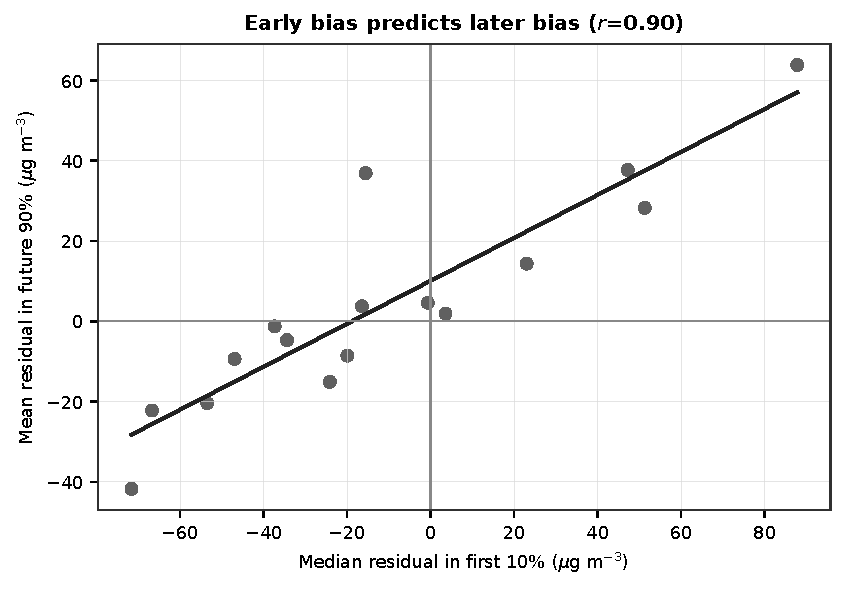
\includegraphics[width=\linewidth]{Figure_10a_TRAQID_bias_relation.pdf}
    \caption{Early-to-future residual relation.}
    \label{fig:bias}
  \end{subfigure}\hfill
  \begin{subfigure}[t]{0.55\textwidth}
    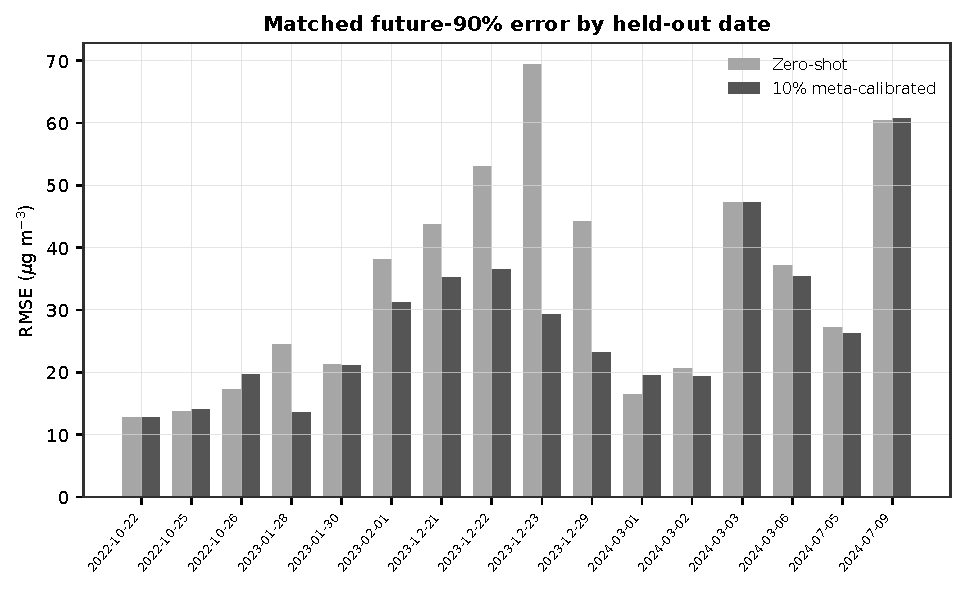
\includegraphics[width=\linewidth]{Figure_10b_TRAQID_calibration_RMSE.pdf}
    \caption{Matched RMSE for every date.}
    \label{fig:date-rmse}
  \end{subfigure}
  \caption{Chronological calibration diagnostics. The association in (a) is
  descriptive; each target-date correction was fitted without that date's
  future targets.}
\end{figure}

\begin{table}[H]
\centering
\caption{Calibration methods on the same future 90\% sequences. Meta-ridge
uses other dates to learn how early bias persists.}
\label{tab:calibration}
\begin{tabular}{lrrrr}
\toprule
Calibration & MAE & RMSE & Pooled \Rtwo & Bias \\
\midrule
None (zero-shot) & 22.67 & 35.28 & 0.371 & -0.68 \\
Direct first-10\% mean offset & 27.96 & 39.48 & 0.212 & -16.52 \\
Direct first-10\% median offset & 28.85 & 40.58 & 0.167 & -19.89 \\
Direct first-10\% affine OLS & 40.89 & 93.32 & -3.404 & -22.05 \\
Meta-ridge early mean & 21.38 & 32.11 & 0.479 & -0.91 \\
Meta-ridge early median & \textbf{21.04} & \textbf{31.77} & \textbf{0.490} & -0.91 \\
\bottomrule
\end{tabular}
\end{table}

Naive direct correction failed because the beginning of a drive was often more
extreme than its remainder. The cross-date ridge mapping learned to shrink this
offset. Date-cluster bootstrap 95\% intervals were MAE 16.43--25.99, RMSE
22.72--40.09 and pooled \Rtwo{} -0.070--0.772 for the calibrated method; the
corresponding zero-shot intervals were MAE 17.92--28.08, RMSE 26.63--43.20 and
pooled \Rtwo{} -0.201--0.640. The width of these intervals prevents a claim of
uniform performance across future dates.

This protocol also requires a functioning roadside \pmfine{} sensor during the
first 10\% of each new drive and a contemporaneous external reference during
the remainder. It is therefore suitable for online sensor/background
calibration or gap filling after warm-up, not sensor-free deployment.

Concentration-stratified analysis exposed the safety-relevant failure mode
(Figure~\ref{fig:traqid-strata}). Calibration reduced RMSE from 109.75 to
95.96 \ugm{} above 150 \ugm, but these 921 high-concentration sequences remained
far harder than observations below 90 \ugm. It also worsened RMSE in the
60--90 \ugm{} band (22.05 to 25.71 \ugm), confirming that a pooled gain did not
improve every regime.

\begin{figure}[H]
  \centering
  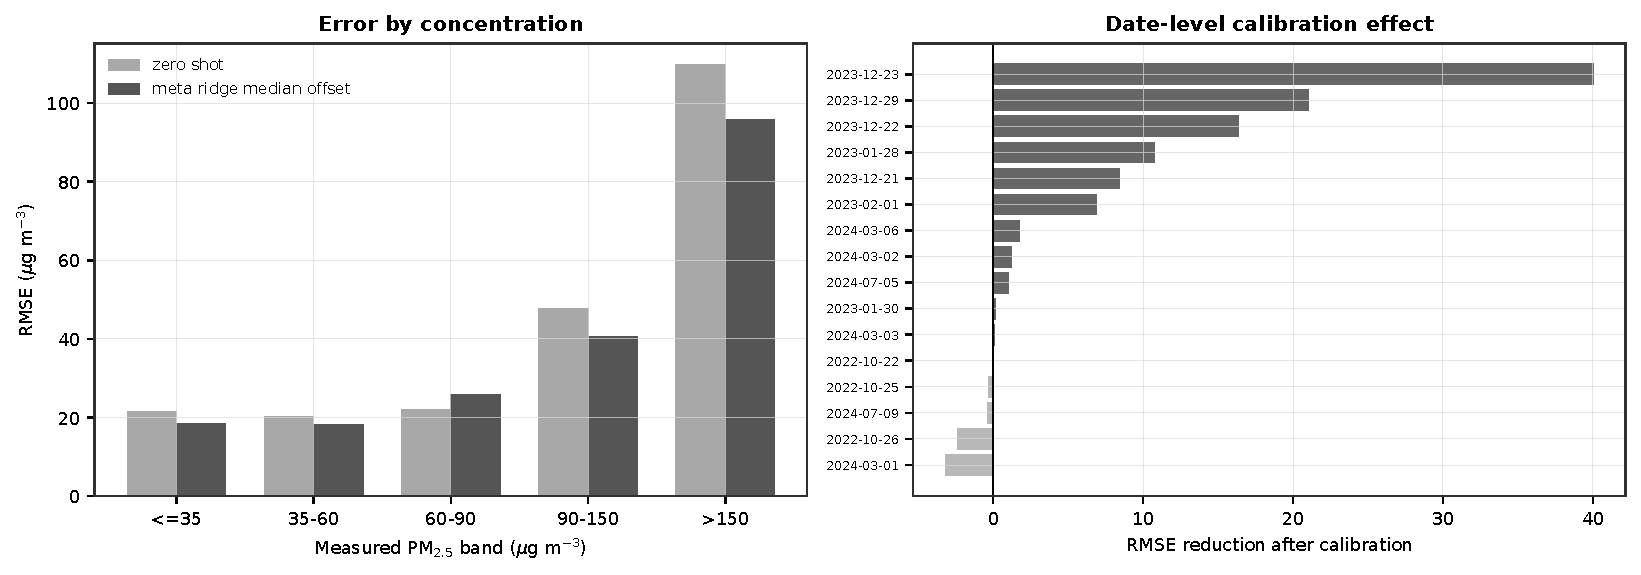
\includegraphics[width=0.98\textwidth]{Figure_11_TRAQID_grouped_sensitivity.pdf}
  \caption{TRAQID robustness analysis. Left: future-90\%
  zero-shot and calibrated RMSE by measured concentration. Right: matched
  date-level RMSE changes; positive bars favour calibration. No model was
  refitted or selected for this analysis.}
  \label{fig:traqid-strata}
\end{figure}

\begin{figure}[H]
  \centering
  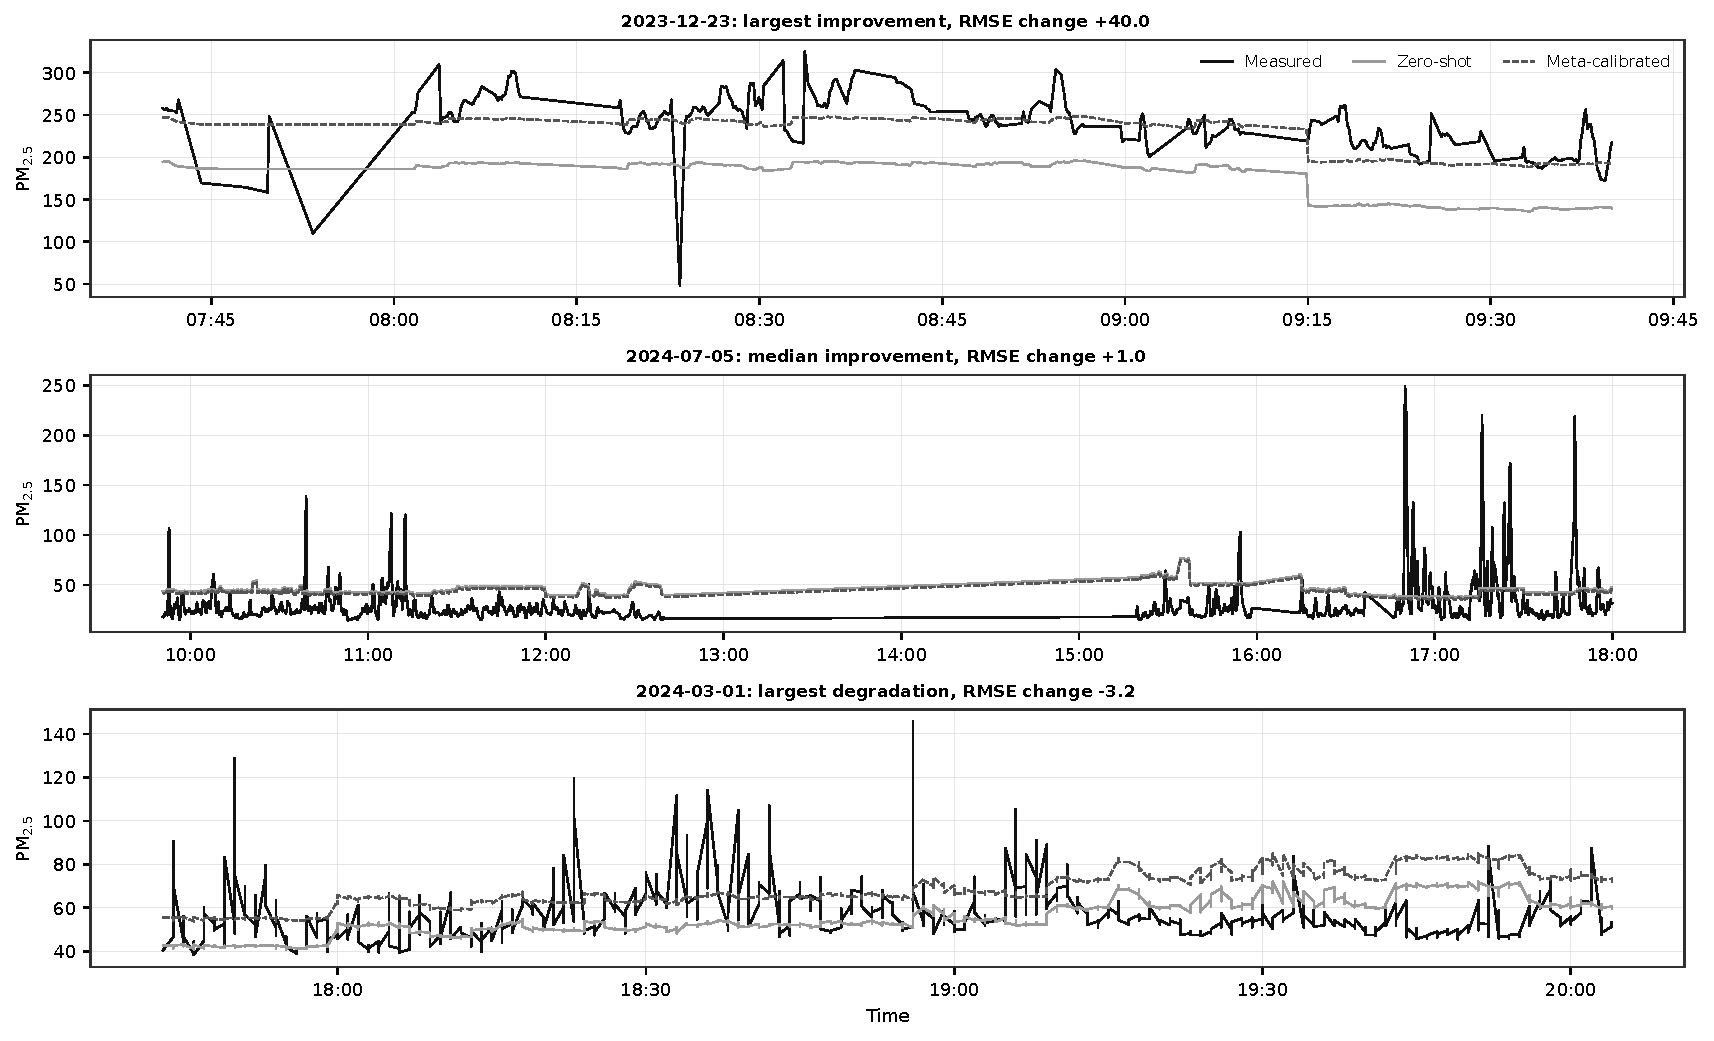
\includegraphics[width=0.98\textwidth]{Figure_12_TRAQID_measured_predicted_examples.pdf}
  \caption{Measured, zero-shot and calibrated time series for the dates with
  the largest RMSE improvement, median improvement and largest degradation.
  Dates were selected mechanically from the paired RMSE differences rather than
  chosen for visual appearance.}
  \label{fig:timeseries}
\end{figure}

\section{Discussion}

\subsection{Validation protocol dominates the apparent result}

The difference between random-window \Rtwo=0.950 and 20-date LODO
\Rtwo=0.188 is not a small degradation caused by one architectural choice. It
is a change in the scientific question. The random protocol asks whether the
model interpolates within a drive when almost every target has appeared in
training context. LODO asks whether relationships learned on other dates
survive a new pollution regime. Reporting only the random score would therefore
mischaracterize deployment capability.

The overlap audit complements rather than invalidates prior image-based work.
Random-sequence results remain useful for reproduction, debugging and
same-distribution interpolation. They become problematic only when interpreted
as evidence of future-date generalisation.

The constructive implication is that model design and validation design cannot
be separated. The random model was implicitly free to recover background state
from adjacent observations; the grouped task removes that shortcut. Supplying
an inference-time background explicitly and restricting the learned model to a
local refinement is therefore a direct response to the failure exposed by the
audit, rather than an unrelated increase in model complexity.

The Taiwan results show why the audit should be paired with a constructive
evaluation rather than treated only as a critique. With dates isolated before
window construction, a background-conditioned model retained
\Rtwo=0.706 over 54 retrospectively defined future dates. With complete sites isolated and fusion
selected inside training sites, pooled \Rtwo{} remained 0.702 and every site
score was positive. The two protocols test different shifts, yet both support
the same design principle. A strong inference-time network background carries
broad spatiotemporal variation, while learned branches estimate a restrained
local departure. The fitted estimators themselves are dataset-specific.

\subsection{Why monitoring-network background and calibration help}

Coarse atmospheric fields cannot reproduce roadside concentration directly,
but they identify the broad aerosol regime. A nearby reference station further
anchors city-scale conditions. The local model then estimates departure from
that anchor. The improvement from reference-only pooled \Rtwo=0.198 to
reference-context local modelling at 0.361 confirms that the learned local
component remains necessary.

The first 10\% of a new date supplies information about sensor/background
offset that atmospheric products do not resolve. Directly applying that early
offset overcorrected because pollution evolved during the drive. Learning the
early-to-later relationship across other dates provided a restrained correction
and improved most dates. This is a practical calibration-assisted task, but it
requires roadside labels during adaptation and a contemporaneous reference
input throughout inference.

The synchronized Taiwan background is conceptually related to CAMS, MERRA-2
and the TRAQID OpenAQ input, but it is local, contemporaneous and multi-site.
It is not target leakage because site $s$ is excluded when predicting site $s$.
It does, however, change the deployment requirement: other network monitors
must report at the target hour. The one-hour-lag ablation (\Rtwo=0.647) shows
that stale observations materially reduce performance, while the single-site
outage audit increased background RMSE by at most 0.20 \ugm. The 0.690
background-only score establishes how much predictive information that
infrastructure already provides; comparisons against it, not against a global
mean, quantify the value of learned context and imagery.

\subsection{Interpretation of the multimodal architecture}

The framework assigns complementary roles to its inputs. Atmospheric products
and synchronized monitors establish the broad pollution state; temporal images
encode visibility and persistent scene appearance; structured road, traffic and
meteorological variables describe local operating conditions. The local model
then learns a restrained departure from the supplied background rather than
reconstructing the entire concentration from imagery alone.

This design was most effective in the fixed Taiwan scenes, where camera geometry
was stable and a synchronized network supplied local background conditions. The
complete model improved the prespecified background on the chronological test
and retained positive performance at every held-out site. Mobile TRAQID posed
a harder shift because route, scene, sensor state and regional pollution changed
together; there the strongest improvement came from combining reference context
with explicit early-date calibration. The two settings therefore demonstrate
how a shared governing formulation can be instantiated with separate models
according to the available sensing infrastructure.

Component-level and exploratory background comparisons are reported in
Appendices~\ref{app:component-audit} and~\ref{app:taiwan-exploratory}. They do
not replace the prespecified frozen evaluations, but identify useful future
extensions: learned spatial background fields, visibility-specific pretraining,
sky/road region separation and domain adaptation selected without target-test
inspection.

\subsection{Limitations, measurement uncertainty and scope}

The study has nine central limitations. First, sequences remain autocorrelated
within grouped dates even when partitions are leakage-safe. Second, the TRAQID
reference-assisted analysis covers 16 dates and one usable OpenAQ station
approximately 4.97 km from the campaign centre; route-specific distance varies,
matching permits gaps up to 90 minutes and four dates lack coverage. The Taiwan
one-hour-lag and single-support-site outage tests quantify background staleness
and redundancy, but matched TRAQID distance/tolerance sensitivity remains a
prospectively specified follow-up rather than an unreported completed analysis.
Third, its 10\% protocol changes
the task from zero-shot prediction to calibration-assisted future-period
prediction. Fourth,
the Taiwan task assumes contemporaneous access to other network sites and is
therefore not camera-only estimation. Fifth, both datasets and the retrospective
Taiwan test period were available during the broader research programme; a new
prospectively frozen campaign is still required for definitive external
confirmation. Retrospective network-model extensions are confined to the
appendix. Sixth, the redistributed Taiwan files used here do not contain
embedded station coordinates, pairwise geometry or monitor instrument
identifiers, so those network characteristics could not be audited directly
from those files. Seventh, the TRAQID target comes from a calibrated SDS011
low-cost sensor and the redistributed Taiwan files omit monitor-model metadata.
Target measurement error, instrument drift and cross-instrument differences are
therefore not propagated into the predictive intervals; reported intervals
quantify sampling variation across dates or sites, not total measurement
uncertainty. Eighth, six held-out sites provide only six independent spatial
clusters. The paired site-cluster interval is reported, but bootstrap repetition
cannot compensate for the small number of spatial units. Ninth, the models
estimate concentration, not chemical source contributions; visual, traffic and
road features are associative proxies.

Grouped bootstraps reflect date or site sensitivity, but 16 TRAQID dates, 54
Taiwan test dates and six Taiwan sites do not represent all cities, instruments,
seasons or camera systems. The grouped intervals and per-group errors should
therefore accompany pooled headline values.

\section{Conclusion}

This study developed and evaluated a leakage-aware multimodal framework that
combines an atmospheric or monitoring-network background with temporal imagery
and structured local context through a reusable sequence-audit, background-
availability, grouped-cross-fitting and uncertainty-reporting workflow. On
TRAQID, the frame audit showed that the
random-window score of \Rtwo=0.950 primarily measured interpolation among
overlapping sequences. Under complete-date evaluation, local-reference
conditioning achieved zero-shot \Rtwo=0.361, while first-10\%
calibration-assisted prediction improved the matched future-90\% result from \Rtwo=0.371 to
0.490 and reduced RMSE by 9.9\%. Mean and median date-wise \Rtwo{} for the
calibrated task were -1.861 and -0.583, with 3 of 16 dates positive; the gain is
therefore useful but not evidence of uniformly stable within-date tracking.

On the six-site Taiwan network, the complete estimator achieved
\Rtwo=0.706, RMSE 6.44 \ugm{} and MAE 4.58 \ugm{} over 7,180 sequences from 54
retrospectively defined future dates, with a positive paired date-bootstrap
improvement over the prespecified network background. Nested leave-one-site-out
evaluation retained pooled \Rtwo=0.702, mean and median site-wise \Rtwo{} of
0.692 and 0.709, and positive \Rtwo{} at all six held-out sites. The site-level
increment over the context model was small and its paired six-site interval
included zero, so Taiwan is interpreted as monitoring-network-assisted local
refinement rather than camera-only estimation. Together, the two datasets
demonstrate a flexible framework in which
background information captures broad pollution state and learned visual and
contextual branches refine the estimate for the local sensing environment.

The broader contribution is a practical, protocol-aware path from shuffled
accuracy to credible multimodal estimation: audit raw context, isolate complete
dates and sites, exclude self-reference, state which background information is
available at inference, and evaluate the full system under the temporal and
spatial shifts it is intended to serve. Grouped uncertainty and component
sensitivity remain essential qualifications and are reported in the appendices.

\section*{Data and software availability}

TRAQID and the Taiwan surveillance-image data are publicly available through
their source publications \citep{kathalkar2024traqid,wang2026unified}.
Analysis software, experiment configurations, split audits and derived tables
are available free of charge at
\url{https://github.com/Kumaryan12/roadside-pm-visual-intelligence}.
The software and derived-result release series used for this manuscript is
archived at Zenodo under the version-independent concept DOI
(\href{https://doi.org/10.5281/zenodo.22121571}{doi:10.5281/zenodo.22121571});
the frozen analysis snapshot is release \texttt{v1.0.3-paper}
\citep{kumar2026roadside}. The software is written in
Python 3.11 and uses PyTorch, scikit-learn, pandas, NumPy, SciPy, Matplotlib,
torchvision and Pillow. It was first released in 2026 and is developed and
maintained by Aryan Satyendra Kumar
(\href{mailto:kumararyan66472@gmail.com}{kumararyan66472@gmail.com}). Release
\texttt{v1.0.3-paper} is distributed at zero cost under the MIT licence and is
approximately 50 MB as a compressed source archive, excluding third-party raw
datasets. It runs on macOS or Linux with a CPU; a CUDA-capable GPU is optional
for neural-network training. Apple Silicon and x86-64 CPU execution are
supported through the Python dependencies; experiments requiring CUDA depend
on a compatible NVIDIA GPU and PyTorch build.
Dependencies are pinned through \path{pyproject.toml} and
\path{requirements.txt}; primary prediction checksums, executable commands,
feature manifests and selection status are listed in \ref{app:provenance}.
The source image datasets are not redistributed because their original licences
and access conditions remain controlling; accession links are provided in their
cited source publications. OpenAQ observations and global atmospheric products
remain subject to their respective providers' access and redistribution terms,
and the repository records retrieval and derivation procedures. This combined
manuscript supersedes
the earlier standalone TRAQID draft, which will not be submitted separately.

\section*{Ethics and data governance}
This study performed secondary analysis of publicly released research
datasets and public environmental observations. No new human participants were
recruited and no attempt was made to identify individuals appearing incidentally
in mobile-road or fixed-camera imagery. The analysis did not use face or licence
plate recognition, identity labels or person-level tracking. Deployment on new
imagery would require jurisdiction-specific privacy review, retention limits
and, where appropriate, de-identification. Use and redistribution of source
data remain governed by the original dataset and service terms.

\section*{CRediT authorship contribution statement}
Aryan Satyendra Kumar: Conceptualization, Methodology, Software, Validation,
Formal analysis, Visualization, Data curation, Writing---original draft, and
Writing---review and editing.

\section*{Competing interests}
The author declares no competing interests.

\section*{Funding}
This research did not receive any specific grant from funding agencies in the
public, commercial, or not-for-profit sectors.

\appendix

\section{Experiment provenance and selection status}
\label{app:provenance}

\begin{table}[H]
\centering
\caption{Provenance of headline and diagnostic results. ``Frozen'' means that
model or correction selection used only declared training/validation groups;
it does not imply prospective collection.}
\begin{adjustbox}{max width=\textwidth}
\begin{tabular}{P{3.0cm}P{4.4cm}P{2.2cm}P{5.2cm}}
\toprule
Result & Primary artifact & Selection status & Permitted interpretation \\
\midrule
TRAQID random \Rtwo=0.950 & Random conditional run and overlap audit & Diagnostic & Contaminated same-distribution interpolation \\
TRAQID 20-date LODO \Rtwo=0.188 & Multi-source LODO predictions & Outer grouped & Zero-shot complete-date performance \\
TRAQID 10\% calibration \Rtwo=0.490 & Chronological calibration predictions and split audit & Outer-safe assisted & Calibrated future-90\% performance \\
TRAQID oracle 0.582--0.663 & Oracle residual analysis & Target-informed & Non-operational diagnostic ceiling \\
Taiwan chronological \Rtwo=0.706 & Chronological reference run & Frozen retrospective & Future-period performance on 54 dates \\
Taiwan LOSO \Rtwo=0.702 & Nested conditioned-image report & Nested outer-site & Spatial transfer across six held-out sites \\
Taiwan learned network 0.740 & Chronological network ablation & Post-hoc & Hypothesis for prospective confirmation only \\
\bottomrule
\end{tabular}
\end{adjustbox}
\end{table}

The baseline sensitivity analysis uses
\path{pipelines/china_surveillance_aqi/analyze_reviewer_baselines.py}
with the frozen chronological predictions, 5,000 complete-date bootstrap
resamples and seed 42. It does not refit the frozen image model. The sequence
manifest, prediction tables, split audit and generated summaries are retained
with the repository workflow; raw third-party imagery is not redistributed.

The TRAQID robustness analysis is implemented by
\path{pipelines/image_embeddings/analyze_traqid_reviewer_metrics.py}. It reads
preserved outer-test predictions only: no model is refitted and no test result
is used for selection. The three primary TRAQID prediction files have SHA-256
prefixes \texttt{7005fee2e774} (20-date LODO), \texttt{7bec2ab0c306}
(reference-assisted LODO) and \texttt{3212eca9e387} (chronological
calibration). The frozen Taiwan chronological prediction file has prefix
\texttt{362e59a70b67}. Complete hashes and deterministic split manifests are
retained beside the run artifacts.

\begin{table}[H]
\centering
\caption{Taiwan monitoring-site metadata and retained availability. Site names
and regional context follow the source publication; codes and counts follow the
redistributed processed manifest. Coordinates and instrument identifiers were
not embedded in the redistributed files.}
\label{tab:taiwan-availability}
\begin{adjustbox}{max width=\textwidth}
\begin{tabular}{lllrrll}
\toprule
Dataset code & Site name & Location context & Rows & Dates & First timestamp & Last timestamp \\
\midrule
48 & Qiaotou & Southern Kaohsiung & 5,533 & 259 & 2019-07-01 19:00 & 2020-04-06 20:00 \\
49 & Renwu & Southern Kaohsiung & 5,952 & 273 & 2019-07-01 19:00 & 2020-04-06 20:00 \\
50 & Fengshan & Southern Kaohsiung & 3,743 & 170 & 2019-10-17 20:00 & 2020-04-06 20:00 \\
51 & Daliao & Southern Kaohsiung & 3,765 & 170 & 2019-10-17 20:00 & 2020-04-06 20:00 \\
52 & Linyuan & Southern Kaohsiung & 5,930 & 271 & 2019-07-01 19:00 & 2020-04-06 20:00 \\
58 & Xiaogang & Southern Kaohsiung & 3,688 & 169 & 2019-10-17 20:00 & 2020-04-06 20:00 \\
\bottomrule
\end{tabular}
\end{adjustbox}
\end{table}

\section{Target-informed TRAQID diagnostic ceilings}
\label{app:oracle}

The following rows use every target from the evaluated date and are therefore
not operational model results. They isolate how much residual error is associated
with date-specific offset and scale.

\begin{table}[H]
\centering
\caption{Achieved reference-assisted performance and target-informed ceilings
on the same 16 complete dates.}
\begin{tabular}{lrrrr}
\toprule
Diagnostic & MAE & RMSE & Pooled \Rtwo & Bias \\
\midrule
Zero-shot reference-context model & 23.94 & 36.23 & 0.361 & 1.04 \\
Oracle date-mean correction & 19.08 & 29.29 & 0.582 & 0.00 \\
Oracle date-affine correction & 15.30 & 26.32 & 0.663 & 0.00 \\
\bottomrule
\end{tabular}
\end{table}

\section{Complete per-date calibration errors}

Table~\ref{tab:perdate} reports the matched future-90\% errors for every date.
No date is omitted. Per-date \Rtwo{} is not used to rank models because several
dates have narrow target variance, making the statistic unstable; MAE, RMSE and
bias are reported consistently for both methods.

\begin{table}[H]
\centering
\caption{Matched future-90\% performance by date.}
\label{tab:perdate}
\begin{adjustbox}{max width=\textwidth}
\begin{tabular}{lrrrrrr}
\toprule
Date & $n$ & Zero MAE & Cal. MAE & Zero RMSE & Cal. RMSE & RMSE change \\
\midrule
2022-10-22 & 1,531 & 11.25 & 11.25 & 12.72 & 12.72 & +0.00 \\
2022-10-25 & 1,003 & 10.19 & 11.23 & 13.73 & 14.04 & -0.31 \\
2022-10-26 & 1,965 & 12.97 & 14.64 & 17.19 & 19.59 & -2.39 \\
2023-01-28 & 993 & 21.45 & 10.52 & 24.42 & 13.62 & +10.79 \\
2023-01-30 & 1,130 & 16.76 & 15.15 & 21.20 & 21.05 & +0.14 \\
2023-02-01 & 1,216 & 24.14 & 28.45 & 38.02 & 31.13 & +6.88 \\
2023-12-21 & 625 & 29.68 & 28.51 & 43.72 & 35.27 & +8.44 \\
2023-12-22 & 651 & 44.42 & 30.31 & 52.94 & 36.57 & +16.37 \\
2023-12-23 & 381 & 65.76 & 20.90 & 69.34 & 29.32 & +40.02 \\
2023-12-29 & 356 & 37.71 & 13.51 & 44.15 & 23.15 & +21.01 \\
2024-03-01 & 963 & 11.59 & 16.10 & 16.38 & 19.55 & -3.17 \\
2024-03-02 & 1,118 & 15.00 & 11.49 & 20.56 & 19.35 & +1.20 \\
2024-03-03 & 1,731 & 29.77 & 30.11 & 47.27 & 47.19 & +0.08 \\
2024-03-06 & 1,434 & 21.09 & 27.82 & 37.20 & 35.44 & +1.76 \\
2024-07-05 & 1,894 & 22.19 & 20.74 & 27.21 & 26.20 & +1.01 \\
2024-07-09 & 1,563 & 38.59 & 39.00 & 60.31 & 60.68 & -0.37 \\
\bottomrule
\end{tabular}
\end{adjustbox}
\end{table}

\section{Calibration split audit}

Every date used the first chronological segment, kept equal timestamps on one
side of the boundary and removed six overlapping sequences. Across 16 dates,
2,129 sequences were used for adaptation, 96 were purged and 18,554 were
tested. The raw-row overlap after purging was zero for every date.

\section{Taiwan held-out-site results}

\begin{table}[H]
\centering
\caption{Nested leave-one-site-out performance of the conservative
conditioned-image model. Image weight $\alpha$ was selected without the outer
test site.}
\label{tab:taiwan-sites}
\begin{tabular}{lrrrrr}
\toprule
Held-out site & $n$ & Selected $\alpha$ & MAE & RMSE & \Rtwo \\
\midrule
48 & 5,006 & 0.24 & 5.530 & 7.228 & 0.655 \\
49 & 5,595 & 0.30 & 4.409 & 5.741 & 0.778 \\
50 & 3,583 & 0.30 & 4.277 & 5.553 & 0.735 \\
51 & 3,619 & 0.14 & 5.758 & 8.022 & 0.534 \\
52 & 5,684 & 0.00 & 5.073 & 6.740 & 0.683 \\
58 & 3,532 & 0.06 & 3.630 & 4.761 & 0.767 \\
\midrule
Pooled & 27,019 & -- & 4.818 & 6.460 & 0.702 \\
\bottomrule
\end{tabular}
\end{table}

\section{Component ablations and fusion sensitivity}
\label{app:component-audit}

The following component results are retained for complete reporting while the
main text emphasizes the prespecified full-framework evaluations. On all 20
TRAQID dates, adding images to the nonvisual MERRA-2 local model increased
pooled \Rtwo{} from 0.180 to 0.188 and reduced RMSE by 0.19 \ugm. On the
16-date reference-covered subset, the reference-context configuration was the
strongest tested variant. These differences show that the balance among
background, imagery and structured context depends on sensing geometry and
background availability.

\begin{table}[H]
\centering
\caption{Component ablation under complete-date TRAQID LODO.}
\label{tab:ablation}
\begin{adjustbox}{max width=\textwidth}
\begin{tabular}{llrrr}
\toprule
Coverage & Local model & MAE & RMSE & Pooled \Rtwo \\
\midrule
20 dates & Nonvisual & 28.69 & 42.34 & 0.180 \\
20 dates & Nonvisual + images & \textbf{28.53} & \textbf{42.14} & \textbf{0.188} \\
20 dates & Nonvisual + structured visual & 29.63 & 42.94 & 0.157 \\
20 dates & Full multimodal & 29.31 & 42.76 & 0.164 \\
\midrule
16 reference dates & Reference context & \textbf{23.94} & \textbf{36.23} & \textbf{0.361} \\
16 reference dates & Reference context + images & 25.37 & 37.65 & 0.310 \\
16 reference dates & Reference context + structured visual & 26.25 & 38.16 & 0.291 \\
16 reference dates & Full multimodal & 26.13 & 38.29 & 0.286 \\
\bottomrule
\end{tabular}
\end{adjustbox}
\end{table}

On the frozen Taiwan chronological test, the context-only stage obtained
\Rtwo=0.685 compared with 0.690 for the prespecified network background, while
the complete conditioned-image model reached 0.706. Under nested LOSO, context
improved the background from 0.689 to 0.699 and the complete estimator reached
0.702. The six-site paired interval for the final increment over context
included zero; this component-level uncertainty does not alter the achieved
performance of the complete estimator but limits claims about any single
modality in isolation.

\section{Exploratory Taiwan network-background extension}
\label{app:taiwan-exploratory}

\begin{table}[H]
\centering
\caption{Exploratory models on the already-inspected Taiwan chronological test
period. Selection used validation only and no test target entered fitting, but
these values require confirmation on a fresh future period.}
\label{tab:taiwan-exploratory}
\begin{adjustbox}{max width=\textwidth}
\begin{tabular}{lrrrr}
\toprule
Model & MAE & RMSE & \Rtwo & Validation-selected weight \\
\midrule
Monitoring-network median & 4.704 & 6.613 & 0.690 & -- \\
Conditioned-image model & 4.580 & 6.442 & 0.706 & 0.116 \\
Lagged spatiotemporal background & 4.290 & 6.100 & 0.736 & 0.346 \\
Learned spatial background & 4.259 & 6.085 & 0.738 & 0.538 \\
Nonnegative ensemble & \textbf{4.234} & \textbf{6.056} & \textbf{0.740} & sums to 1 \\
\bottomrule
\end{tabular}
\end{adjustbox}
\end{table}

\section{Protocol-aware literature context}

\begin{table}[H]
\centering
\caption{Representative published image-based results. Values are not directly
rankable across datasets or split protocols.}
\label{tab:literature}
\begin{adjustbox}{max width=\textwidth}
\begin{tabular}{P{2.5cm}P{3.2cm}P{3.0cm}P{2.4cm}P{2.2cm}P{3.4cm}}
\toprule
Study & Inputs & Split protocol & Target & Reported \Rtwo & Interpretation \\
\midrule
Wang et al.~\citep{wang2024surveillance} & Surveillance image sequences & Random two-fold sequence CV & \pmfine{} & 0.940 & Overlapping-sequence risk \\
Luo et al.~\citep{luo2020cnn} & Images + weather/time & Study-specific & \pmfine{} & 0.850 & Temporal isolation differs \\
Liu et al.~\citep{liu2024trafficcamera} & Fixed camera + reference monitor & Chronological study-specific & Hourly \pmfine{} & 0.980 & Fixed-scene task \\
PM25\-Vision~\citep{han2026pm25vision} & Global street images & Random image split & Daily AQI label & 0.550 & Different target and scale \\
TRAQID, this work & T=7 multimodal & Random overlapping windows & Roadside \pmfine{} & 0.950 & 99.90\% context leakage \\
TRAQID, this work & Reference context + 10\% adaptation & Complete-date + purged future 90\% & Roadside \pmfine{} & 0.490 & Calibration-assisted \\
Taiwan, this work & Other-site background + conditioned images & Chronological 54-date test & \pmfine{} & 0.706 & Frozen retrospective test \\
Taiwan, this work & Same framework, inner-CV fusion & Nested leave-one-site-out & \pmfine{} & 0.702 & Six unseen sites \\
\bottomrule
\end{tabular}
\end{adjustbox}
\end{table}

\section*{Declaration of generative AI and AI-assisted technologies in the
writing process}
During preparation of this work, the author used OpenAI ChatGPT and Codex to
assist with language editing, manuscript organisation, code review and drafting
reproducible plotting code. The author reviewed and verified all AI-assisted
material, analyses, references and code and takes full responsibility for the
content of the publication. No AI-generated primary observational data or
primary research images were used. Quantitative figures were regenerated
deterministically from preserved observations, split manifests and prediction
tables. The graphical abstract was rendered from editable, author-verified
TikZ/LaTeX geometry and mathematical text; no text-to-image or generative image
model was used.

\section*{Acknowledgements}
The author thanks Sreejith Chakrapani and Navaneethakrishnan V. for research
discussions and technical guidance during the broader project.

\bibliographystyle{elsarticle-harv}
\bibliography{references}

\end{document}
